\chapter{Zero-inflated models}

% \begin{abstract}
\noindent We consider variational inference for zero--inflated Poisson regression models using a latent
variable representation. The model is extended to include random effects which allow simple incorporation of
spline and other modelling structures. Several variational approximations to the resulting set of models are
presented, including a novel approach based on the inverse covariance matrix rather than the covariance matrix
of the approximate posterior density for the random effects. This parameterisation improves upon the
computational cost and numerical stability of previous methods. We demonstrate these approximations on
simulated and real data sets.
% \end{abstract}
 
% \noindent Keywords: Approximate Bayesian inference ; mixed model ; Markov chain Monte Carlo ; Stan ; penalized splines.

% \joc{
% 	Comments: 
% 	\begin{itemize}
% 		\item Need to organize in terms of a flow of ideas. What are we approximating?		      		      		      		      
% 		\item I believe that we are using a semiparametric mean field variational Bayes approach discussed by Rohde \& Wand (2015).
% 		      However, I am not sure that we are using the their formalisms. (see page 3-6 of Rohde and Wand 2015).
% 	\end{itemize}	
% }

\section{Introduction}
\label{sec:introduction}

% \mgc{This section is too short}
Count data with a large number of zero counts arises in many areas of application, such as data arising from
physical activity studies, insurance claims, hospital visits or defects in manufacturing processes. Zero
inflation is a frequent cause of overdispersion in Poisson data, and not accounting for the extra zeroes may
lead to biased parameter estimates. These models have been used for many applications, including defects in
manufacturing in \cite{lambert1992}, horticulture in \cite{BIOM:BIOM1030} and \cite{BIOM:BIOM1030}, length
of stay data from hospital admissions in \cite{BIMJ:BIMJ200390024}, psychology in \cite{JOFP:rethink},
pharmaceutical studies in \cite{Min01042005}, traffic accidents on roadways in \cite{Shankar1997829} and
longitudinal studies in \cite{LeeWangScottYauMcLachlan2006}.

The strength of this approach derives from modelling the zero and non-zero count data seperately as a mixture
of distributions for the zero and non-zero components, allowing analysis of both the proportion of zeroes in
the data set and the conditions for the transition from zero observations to non-zero observations. When
combined with a multivariate mixed model regression framework, an extremely rich class of models can be fit
allowing a broad range of applications to be addressed. Often the transition from zero to non-zero has a
direct interpretation in the area of application, and is interesting in its' own right.

Bayesian estimation methods for zero-inflated models was developed in \cite{Ghosh2006} using MCMC implemented
with WinBUGS, and in \cite{Vatsa2014} using a Variational Bayes solution to the inverse zero- inflated
Poisson regression problem. While simple forms of these models are easy to fit with standard  maximum
likelihood techniques, more general models incorporating random effects, splines and missing data  typically
have no closed form solutions and hence present a greater computational challenge to fit.

In this chapter, we build upon the earlier work on Bayesian zero-inflated models by \cite{Ghosh2006} and
\cite{Vatsa2014}. While simple forms of these models are easy to fit with standard maximum likelihood
techniques, more general models incorporating random effects, splines and missing data typically have no
closed form solutions and hence present a greater computational challenge to fit.

Fitting these models is typically done with Monte Carlo Markov Chain techniques, but these techniques can be
computationally intensive and prone to convergence problems.  Other fitting methods such as the Variational
Bayes approach above can be inflexible, not allowing complicated models incorporating random effects, splines
and missing data.

% This writing doesn't flow well, needs to be improved.
Recently, several stochastic Variational Bayes approaches to approximation problems of this type have emerged.
\cite{Gershman2012} used a uniform weighted mixture of isotropic Gaussians to approximate complex posterior
distributions. The variational lower bound is approximated with first and second-order Taylor series
expansions, and then optimised with L-BFGS.
In \cite{Kingma2013}, the expectations in the expression for the variational lower bound are approximated
using Monte Carlo integration. The variational lower bound is reparameterised in terms of an auxillary
noise variable such as a standard normal, to reduce the variance of the Monte Carlo estimate.
\cite{Tan2018} takes an approach closest to the one we will adopt, using a Gaussian Variational Approximation.
By parameterising the covariance matrix of the Gaussian using Cholesky
factors of the precision matrix, the covariance matrix is guaranteed to be sparse due to the conditional
independence between fixed and random effects of the mixed model. The variational lower bound can be rewritten
so that it does not depend on the variational parameters. 
By making a transformation in terms of a noise variable to standardise the variational parameters,
efficient gradient estimators can be derived, then estimated using subsampling of the data set. Sampling
from the fixed normal distribution on each iteration rather than a multivariate normal depending on the
variational parameters in the current iteration reduces the variance of the estimator.
Subsampling of the data set and sampling from the noise variable make the fitting algorithm doubly stochastic.

Other approximate Bayesian inference techniques exist in the literature, such as
Laplace approximation \cite{Tierney1986}/ integrated nested Laplace approximation \cite{Rue2009} and Expectation Propagation \cite{Minka2013}, and these have been applied to the problem of fitting
count models
\cite{Barber2016}
\cite{KimWand2017}.
But Expectation Propagation requires very difficult algebra to complete the derivations required for the
updates, and is slow to compute. And Laplace approximation relies on a Gaussian approximation to the
log-likelihood found by Taylor expanding around the mode, which performs poorly when the true posterior is
not symmetric, as is the case for Poisson regression models.

We build upon a latent variable representation of these models to allow a tractable semiparametric mean field
Variational Bayes approximation to be derived. Semiparametric Mean Field Variational Bayes is an approximate
Bayesian inference method as detailed in \cite{Ormerod2010} and \cite{Rohde2015}, which allows us to fit
close approximations to these models using a deterministic  algorithm which converges much more quickly.

We allow a flexible regression modelling approach incorporating both fixed and random effects by using a
Gaussian Variational Approximation as defined in \cite{Ormerod2012} on the regression parameters to allow a
non- conjugate Gaussian prior to be used, making the resulting Gaussian posterior distribution of the
regression parameters easy to interpret. We adopt a Mean Field  Variational Bayes (VB) approach on the other
parameters in the model to derive the rest of the approximation.

% This makes sense in a paper, but not in a thesis chapter.
The focus of this chapter is on developing methods of fitting flexible ZIP regression models accurately, and
showing the advantages of our methods to previously presented methods. We also investigate stability problems
that can arise when using naive versions of these methods, and the modifications to the fitting methods we
devised to mitigate these problems. In Section \ref{sec:model} we define our model and provide a framework for
our approach incorporating regression modelling and random effects. In Section \ref{sec:gaussian} we focus on
several approaches to fitting the Gaussian component of our model. In Section \ref{sec:param}, we present new
parameterisations for use in these algorithms which offers substantial advantages in accuracy, numerical
stability and computational speed. In Section \ref{sec:results} we perform numerical experiments on simulated
data which show how our approach offers computational advantages over existing approaches -- in terms of both
speed and stability. In Section \ref{sec:application} we show an application of our pure Poisson model fitting
method to a hierarchical model studying the effect of ethnicity on the rate of police stops, and an
application of our zero-inflated Poisson model fitting method to a multi-level longitudinal study of pest
control in apartments. Finally, in Section \ref{sec:discussion} we conclude with a discussion of the results.
An appendix contains details of the derivation of the variational lower bound for our model.

\section{Zero--inflated models}
\label{sec:model}

In this section we present a Bayesian zero-inflated Poisson model for count data with extra zeroes. After
introducing the latent variable representation of Bayesian zero-inflated models, we first extend this to a
model incorporating fixed effects regression modelling, and extend the model again to a more flexible mixed
model approach incorporating both fixed and random effects.

\subsection{Modelling zero-inflated Poisson data}

We consider a sample of counts $y_i$, $1 \le i\le n$, where there are an excessive number of zeros for a
Poisson model, but the sample is otherwise well--modelled by a Poisson distribution. There are two main
parameterizations for modelling such data. The first approach models the probability of a zero by $\rho$ and
adjusts for counts greater than zero. This model uses the probability distribution specified in
Equation (\ref{eq:zero_infl_first_param}).

\begin{equation}
\label{eq:zero_infl_first_param}
	P(Y_j = y_i) = \left\{ \begin{array}{ll}
	\rho + e^{-\lambda},  & y_i = 0 \\
	\left( \frac{1 - \rho}{1 - e^{-\lambda}} \right) \frac{\lambda^{y_i} e^{-\lambda}} {y_i!},  &y_i \ge 1.
	\end{array} \right.
\end{equation}

A second approach using latent variables views the data as the product of two data--generating processes, a
Bernoulli process that determines whether the data is definitely zero, and a second process where data is
generated from a Poisson distribution which may be zero.

Note that this allows zeros to be generated from the model in one of two ways -- either from the Bernoulli
process generating a zero or from the Bernoulli process generating a Poisson sample which is then zero. A
latent variable representation of this parameterization introduces the latent variables $r_i$ which equal $1$
when $y_i>0$ and $0$ otherwise. This leads to the specification for the probability distribution used in
Equation (\ref{eq:zero_infl_second_param}).

\begin{equation}
\label{eq:zero_infl_second_param}
\begin{array}{rl}
	P(Y_i=y_i|r_i) = & \frac{\exp(-\lambda r_i)(\lambda r_i)^{y_i}}{y_i!} \quad \mbox{and} \\
	r_i \sim & \mbox{Bernoulli}(1-\rho)
\end{array}
\end{equation}

\noindent where $\text{Bernoulli}(\pi)$ denotes the probability distribution $\pi^k (1 - \pi)^{1-k}$.

Let $p$ be the dimension of the space of fixed effects, $m$ be the number of individuals in the random effects
and $b$ be the block size for each of those individuals. We use $\vone_p$ and $\vzero_p$ to denote the $p
\times 1$ column vectors with all entries equal to 1 or 0, respectively.

Let $\vy$ be the $n \times 1$ vector. The norm of a column vector $\vv$, defined to be $\sqrt{\vv^\top \vv}$,
is  denoted by $\|\vv\|$. For a $p \times 1$ vector $\va$, we let $\diag{(\va)}$ denote the $p \times p$
matrix with the elements of $\va$ along its' diagonal.

We denote the design matrix of fixed effects with dimensions $n \times p$ as $\mX$ is , and the design matrix
of random  effects with dimensions $n \times m b$ as $\mZ$. The combined design matrix $\mC$ is formed by
appending the columns of $\mX$ to the columns of $\mZ$, giving $\mC = [ \mX, \mZ ]$.

Let $\vtheta$ is the vector of all parameters.
Let $\vbeta$ be the $p \times 1$ column vector of fixed
effects, and $\vu$ the $m b \times 1$ column vector of random effects. $\vnu$ is the
concatenation of these vectors $[\vbeta^\top, \vu^\top]$.
% Let $\vp$ be the $n \times 1$ column vector of probabilities that each observation in $\vy$ is
% non-zero.

Let $\mSigma$ be the covariance matrix of the random effects $\vu$,
and 
$\mPsi$ the covariance matrix prior on $\mSigma$.
These matrices are all of dimension $(p + m b) \times (p + m b)$.

$\text{expit}(x)$ denotes the function $\tfrac{1}{1 + \exp(-x)}$ which is the inverse of the logit
function.

We can extend the model naturally to a multiple covariate regression model by using a log link function on the
response variable and replacing the parameter $\lambda$ in the model above with $\vx_i^\top \vbeta$ to specify
the mean, where $\vx_i,\vbeta \in \R^p$, with $\vx_i$ the vector of observed predictors and $\vbeta$ the
vector of regression coefficients. Letting $\vr = (r_1,\ldots,r_n)$, the model becomes

\begin{equation*}%\label{eq:main}
	\begin{array}{rl}
		\log p(\vy|\vr, \vbeta) 
		    & = \vy^\top \mR (\mX\vbeta)                           
		- \vr^\top \exp{(\mX\vbeta)} 
		- \vone^\top \log{\Gamma{(\vy + \vone)}}, \quad \mbox{ and }\\ [1ex]
		r_i | \rho & \sim \text{Bernoulli}(1-\rho), \quad 1 \leq i \leq n \\
	\end{array}
\end{equation*}

\noindent where $\mX$ is the $n\times p$ matrix whose $i$th row equals $\vx_i$ and $\mR = \diag{(\vr)}$.

\subsection{Extending to mixed models, incorporating random effects}

To be able to construct multivariate models with as much generality as possible, we wish to specify the full
model as a General Design Bayesian Generalized Linear Mixed Model, as in \cite{Zhao2006}. This allows for a
very rich class of models, which can incorporate such features as random intercepts and slopes, within-subject
correlation and smoothing splines, as in \cite{Wand2008}, into our models.

The zero-inflated model regression model introduced above can be extended to a flexible mixed model by
incorporating the latent variable $\vr$ which controls the mixture of the zero and non-zero components from
the zero-inflated model above into a Poisson mixed model likelihood.

When the indicator $\vr_{ij} = 0$, the likelihood is $1$ for $\vy_{ij} = 0$ and $0$ for all $\vy_{ij} > 0$,
and when the indicator $\vr_{ij} = 1$, the likelihood is a Poisson mixed model regression likelihood for
$\vy_{ij}$. $\vr_{ij}$ is a Bernoulli indicator with probability $\rho$, allowing a proportion of zero-
inflation in the observed data to be specified.

The $j$th predictor/response pair for the $i$th group is denoted by $(\vx_{ij}, \vy_{ij}), 1 \leq j \leq n_i, 1 \leq i \leq m$, where $\vx_{ij} \in \R$, and the $\vy_{ij}$ are nonnegative integers.

For each $1 \leq i \leq m$, define the $n_i \times 1$ vectors $\vy_{ij} = [\vy_{i 1}, \ldots, \vy_{i
n_i}]^\top$ as the response vector. Vectors $\vy_1, \ldots, \vy_m$ are assumed to be independent of each other.

We develop a zero-inflated regression model incorporating both fixed effects $\vbeta$ and random effects
$\vu$. The log-likelihood for one observation is then

$$
	\begin{array}{rl}
		\log p(\vy_{ij} | \vr_{ij}, \vbeta, \vu) & = \vy_{ij} \vr_{ij} (\vx_i^\top \vbeta + \vz_{ij}^\top \vu) - \vr_{ij} \exp (\vx_{ij}^\top \vbeta + \vz_{ij}^\top \vu) - \log \Gamma (\vy_{ij} + 1), \\
		\vr_{ij} | \rho                  & \sim \text{Bernoulli}(\rho), 1 \leq i \leq m, 1 \leq j \leq n, \text{ and }                                                              \\
		\rho                        & \sim \text{Beta}(\alpha, \beta).                                                                                              \\
	\end{array}
$$

\noindent We now extend this to multiple observations. Let $\mC = [\mX, \mZ]$ and $\vnu = [\vbeta^\top, \vu^\top]^\top$. The multivariate model with multiple observations is then
$$
%\label{eq:main}
	\begin{array}{rl}
		\log{p(\vy|\vr, \vbeta, \vu)} & = \vy^\top \mR (\mC\vnu) - \vr^\top \exp{(\mC\vnu)} - \vone^\top \log{\Gamma{(\vy + \vone)}}, \quad \mbox{ and } \\ [1ex]
		r_i                           & \sim \text{Bernoulli}(\rho), 1 \leq i \leq n                                                                     \\
	\end{array}
$$

% \joc{(The prior structure will depend on the structure of the random effects model)}
\noindent with priors
\begin{align*}
	\log{p(\mSigma_{\vu \vu})} & = \text{Inverse Wishart}(\mPsi, v),    \\
	\rho                       & \sim \Beta(\alpha, \beta),             \\
	\vbeta|\sigma^2_\vbeta     & \sim \N_p(\vzero, \sigma^2_\vbeta \mI) \text{ and } \\
	\vu|\mG       & \sim \N_{mb}(\vzero, \mG)              
\end{align*}

\noindent where $\mX$ is $n \times p$, $\mZ$ is $n \times mb$ and $\mSigma_{\vu \vu}$ is $mb \times mb$ and
$\mPsi$ is $b \times b$. The covariance of $\Cov(\vu) \equiv \blockdiag_{1 \leq i \leq m} (\mSigma) \equiv
\mI_m \otimes \mSigma$. $\text{Inverse Wishart}(\mPsi, v)$ denotes the probability distribution
$$\tfrac{|\mPsi|^\frac{v}{2}}{2^{\frac{vp}{2}} \Gamma_p{\left(\tfrac{v}{2}\right)}} |\mX|^{-\tfrac{v + p + 1}{2}}
\exp{\left\{-\tfrac{1}{2} \tr{(\mPsi \mX^{-1})}\right\}}$$ where $\Gamma_p{(x)}$ denotes the multivariate gamma function and $\tr$
is the trace function.

The covariance matrix of random effects $\mSigma$ will depend on the mixed model being fit. In the random
intercept case, $\mSigma = \sigma_u^2 \mI$ while in the random slopes case
\[
	\mSigma = 
	\begin{pmatrix}
		\sigma_{\vu_1}^2                                 & \rho_{\vu_1 \vu_2} \sigma_{\vu_1} \sigma_{\vu_2} \\
		\rho_{\vu_1 \vu_2} \sigma_{\vu_1} \sigma_{\vu_2} & \sigma_{\vu_2}^2                                 
	\end{pmatrix}
\]
where $\sigma_{\vu_1}^2$ is the variance of the random intercepts, $\sigma_{\vu_2}^2$ is the variance of the
random slopes and $\rho_{\vu_1 \vu_2}$ is the correlation between the random intercepts and random slopes.

% \joc{Shouldn't we specify the structure of $\mSigma_{\vu \vu})$ later
% which is different for the random intercept, slope and spline cases?}
% \joc{(Perhaps it is wroth spelling out all of the various random effects structures that we will be using. Consider templating from Zhao \etal (2006).))}

In the spline case, we use the cubic spline basis $1$, $x$, $x^3$, $(x - \kappa_1)^3_+$, \ldots, $(x -
\kappa_K)^3_+$, where $K$ is the number of knots. $\mSigma$ is a $K + 2$ banded matrix, where $K$ is the
number of knots. Banded matrices are highly sparse, and matrix operations can be performed on them in
$\BigO(n)$ time. The matrix $\mSigma$ is symmetric, with contents
\[
	\mSigma =
	\begin{pmatrix}
		\sigma^2_{\text{intercept}} & \ldots                      &                             &                               &                                          & \text{symmetric}              \\
		\rho_{\text{intercept} x} & \sigma^2_x & \ldots\\
		\rho_{\text{intercept} x^2} & \rho_{x x^2} & \sigma^2_{x^2} & \ldots \\
		\rho_{\text{intercept} x^3} & \rho_{x x^3} & \rho_{x^2 x^3} & \sigma^2_{x^3} & \ldots \\
		0                           & \rho_{x (x - \kappa_1)^3_+} & \rho_{x^2 (x-\kappa_1)_+^3} & \rho_{x^3 (x - \kappa_1)_+^3} & \sigma^2_{(x - \kappa_1)_+^3}            & \ldots                        \\
		0                           & 0                           & \rho_{x^2 (x-\kappa_2)_+^3} & \rho_{x^3 (x-\kappa_2)_+^3}   & \rho_{(x-\kappa_1)_+^3 (x-\kappa_2)_+^3} & \sigma^2_{(x - \kappa_2)_+^3} \\
		0 & 0 & 0 & \rho_{x^3 (x - \kappa_3)_+^3} & \rho_{(x - \kappa_1)_+^3 (x - \kappa_3)_+^3} & \rho_{(x - \kappa_2)_+^3 (x - \kappa_3)_+^3}
	\end{pmatrix}.
\]

\subsection{Variational Bayes Approximation to the Zero-Inflated Poisson model}

We choose a factored variational approximation for the model of the form 
\[
	q(\vnu, \sigma_{\vu}^2,\vr_0, \rho) = q(\vnu) q(\mSigma_{\vu \vu}) q(\vr_0) q(\rho)
\]

\noindent 
where we define $\vr_0 = \{ r_i : y_i = 0 \}$. \\
% The distributions we select are?
$q(\vnu) = \N(\vmu, \mLambda)$, \\
$q(\sigma_{\vu}^2) = \text{Inverse Wishart}\left(\mPsi + \sum_{i=1}^m (\vmu_i \vmu_i^\top + \mLambda_{\vu_i \vu_i}), v + m \right)$ \mbox{and } \\
$q(r_i) = \text{Bernoulli}{(p_i)}$ with
$$p_i = 
\begin{cases}
\text{expit}\left\{ \psi{(\alpha_{q(\rho)})} - \psi{(\beta_{q(\rho)})} - \exp{(c_i^\top\vmu + \frac{1}{2} c_i^\top \mLambda c_i)} \right\},& \text{ when } \vy_i = 0\\
1,& \text{ otherwise.}
\end{cases}$$

%$\propto \exp{\left \{-r_i \bE_{-r_i} [\exp{(c_i^\top\vnu)}] + r_i [\psi(\alpha_\rho) - \psi(\beta_\rho)] \right \} }.\\$

The optimal approximation is given in Equation (\ref{eq:optimal_approximation})
% \joc{(reword: the ``optimal approximation'' might be called the true posterior)}
for $\vr$ is
\begin{equation}
\label{eq:optimal_approximation}
\begin{array}{rl}
	q(\vr) & \propto \exp \left \{ \bE_{-q(\vr)}\vy^\top\mR(\mC\vmu) - \vr^\top\exp{(\mC\vnu)}-\frac{1}{2} \vnu^\top \mSigma_{\vu \vu} \vnu \right \}                                                  \\ [1ex]
	       & = \exp{ \left[ \vy^\top\mR\mC \vmu - \vr^\top \exp{\{\mC \vmu + \frac{1}{2} \text{diag}(\mC \mLambda \mC^\top)\}} - \frac{1}{2} \vmu^\top \mD \vmu - \frac{1}{2} \text{tr}(\mLambda \mD ) \right] } 
\end{array}
\end{equation}
\noindent where $\mD = \left\{ (\mPsi + \sum_{i=1}^m \vmu_i \vmu_i^\top + \mLambda_{\vu_i\vu_i}) / (v - p - 1) \right\}^{-1}$. 

We observe that this expression is close in form to the likelihood of a Poisson regression model with random
effects. Poisson regression models are non-conjugate with normal priors, and hence the mean field updates for
the regression parameters do not have closed form expressions. But by assuming a multivariate normal
distribution for the regression co-efficients parameterised by $\vmu$ and $\mLambda$, the model can still be
fit using a Gaussian Variational Approximation for $\vbeta$ and $\vu$ jointly. Techniques for efficiently
fitting these models are described in \cite{Ormerod2012}, \cite{Challis2013} and \cite{Opper2009}. Gaussian
variational approximations have also been shown to have good asymptotic properties in \cite{Sinica2017}. The
model can be fit using Algorithm \ref{alg:algorithm_one} below.

\begin{algorithm}
	\caption[Algorithm 1]{Iterative scheme for obtaining the parameters in the
		optimal densities $q^*(\vmu, \mLambda)$, $q^*(\mSigma_{\vu \vu})$ and $q^*(\rho)$}
	\label{alg:algorithm_one}
	\begin{algorithmic}
		\REQUIRE{$\alpha_{q(\rho)} \leftarrow \alpha_\rho + \vone^\top\vp, p_{q(\mSigma_{\vu \vu})} \leftarrow p + 1$} \\[1ex]
		\WHILE{the increase in $\log{\underline{p}}(\vy;q)$ is significant}
		% \vmu, \mLambda
			\STATE Optimise $\vmu$ and $\mLambda$ using $\vy, \mC, \vp$ and $\mSigma_{\vu \vu}$ \\[1ex]
			% \vp
			\STATE $\beta_{q(\rho)} \leftarrow \beta_\rho + n - \vone^\top\vp$ \\[1ex]
			\STATE $\veta \leftarrow -\exp \left \{ \mC \vmu + \frac{1}{2} \diag{(\mC\mLambda\mC^\top)} \right \} + (\psi{(\alpha_{q{(\rho)}})} - \psi{(\beta_{q{(\rho)}})}) \vone_n$ \\[1ex]
			\STATE $\vp_{q(\vr_0)} \leftarrow \text{expit}{(\eta)}$ \\[1ex]
			% \mSigma_{\vu \vu}
			\STATE $\mPsi_{q(\mSigma_{\vu \vu})} \leftarrow \mPsi + \sum_{i=1}^m (\vmu_i \vmu_i^\top + \mLambda_{{\vu}_i {\vu}_i})$ \\[1ex]
			\STATE $\mSigma_{\vu\vu} \leftarrow \{\mPsi_{q(\mSigma_{\vu \vu})}/(v - d - 1)\}^{-1}$
		\ENDWHILE
	\end{algorithmic}
\end{algorithm}
						
\section{Optimising the Gaussian Part of the Model}
\label{sec:gaussian}

The most computationally and numerically difficult part of Algorithm \ref{alg:algorithm_one} above is
optimising the mean and covariance of the Gaussian approximation to the regression co-efficients $[\vbeta,
\vu]^\top$. In this section, we compare the accuracy, stability and speed of four different algorithms for
fitting the Gaussian component of our model, $q(\vmu, \mLambda)$ in Algorithm \ref{alg:algorithm_one}.  We
compare these approaches for accuracy, computational complexity and stability.

Our first attempts at implementation of some of these algorithms were prone to numerical stability problems
when initialised from some starting points. We also discuss the modifications we made to these algorithms to
enhance their numerical stability.
	
\subsection{Laplace-Variational Approximation}
The Laplace-Variational Approximation method is based on Laplace's method of approximating integrals, as
introduced in Section \ref{sec:laplace_approximation}. The variational lower bound  is approximated by a
Gaussian centred at its' mode.

% Laplace's method of
% approximation uses the second order Taylor expansion of the full log likelihood of the  model around the
% mode to find a Gaussian approximation to the full posterior. Taylor expanding the full log likelihood
% once around the mode yields the following approximation.
This yields the approximation to the variational lower bound in (\ref{eq:laplace_variational_lower_bound}).
% The algorithm is very quick to execute, but the resulting approximate posterior
% distributions are not as accurate as those produced by the other algorithms considered in this article.
% NR
% Detail the function and its derivatives
\begin{equation}
\label{eq:laplace_variational_lower_bound}
\begin{array}{ll}
	\log \underline{p}(\vmu, \mLambda; \vy) \approx \vy^\top\mP\mC\vmu - \vp^\top\exp \left (\mC \vmu \right ) - \tfrac{1}{2} \vmu^\top \mSigma^{-1} \vmu. 
\end{array}
\end{equation}
		
\noindent This expression can be iteratively optimised with respect to $\vmu$ and $\mLambda$ using the
Newton-Raphson method, with the derivatives for $\vmu$ and $\mLambda$ given in Appendix
\ref{sec:appendix_derivatives_laplace}. The steps of the algorithm are shown in Algorithm \ref{alg:laplace_alg}.
		
Upon implementing the algorithm and performing numerical experiments, we observed numerical issues which had to be dealt with in 
order for the algorithm to successfully complete.
% Describe the iteration
We implemented checks for error conditions, and steps to recover from the error conditions should
they arise.

If during an iteration of the Laplace-Variational approximation algorithm the inversion  of $\mLambda$
fails, or the diagonal elements of $\mLambda$ become negative when $\mLambda$ must be positive-definite,
then $\vmu$ and $\mLambda$ were reverted to the previous iteration's $\vmu$ and $\mLambda$ values and
the algorithm was terminated.

If after calculating the gradient of the Gaussian Variational lower bound with respect to $\vmu$, any of
its' elements were NaN or $\infty$, then $\vmu$ and $\mLambda$ were reverted to the previous iteration's
$\vmu$ and $\mLambda$ values and the algorithm was terminated.
		
\begin{algorithm}
	\caption{Laplace scheme for optimising $\log \underline{p}(\vmu, \mLambda; \vy)$}
	\label{alg:laplace_alg}
	\begin{algorithmic}
		\REQUIRE $\mH \leftarrow [- \mC^\top \text{diag}(\vp e^{(\mC \vmu)}) \mC - \mSigma^{-1}]^{-1}$.
		% Fit \vmu, \mLambda using Laplace approximation
		\WHILE{the increase in $\log \underline{p}(\vmu, \mLambda; \vy)$ is significant}
		% \vmu, \mLambda
		\STATE $\mLambda \leftarrow \left \{\mP \mC^\top \text{diag}(\exp{(\mC \vmu)}) \mC + \mSigma^{-1} \right \}^{-1}$ \\ [1ex] 
		If $\mLambda$ cannot be inverted, or any diagonal element of $\mLambda$ is negative, revert to previous
		$\mLambda$ and break \\ [1ex]
		\STATE $\mH
		\leftarrow [- \mC^\top \text{diag}(\vp e^{(\mC \vmu)}) \mC - \mSigma^{-1}]^{-1}$ \\ [1ex]
		If any element of $\mH$ is NaN or $\infty$,
		break
		\STATE $\vmu \leftarrow \vmu + \mLambda g$ \\ [1ex]
		\ENDWHILE
	\end{algorithmic}
\end{algorithm}
		
\subsection{Gaussian Variational Approximation}
		
% Detail techniques used for fitting models.
The full variational likelihood for a Generalised Linear Mixed model is computationally difficult to compute,
requiring the evaluation of a high dimensional integral. However, \cite{Ormerod2012} devised an accurate
approximation to the full variational likelihood, the Gaussian Variational Lower Bound, which only requires
the evaluation of a substantially simpler univariate integral.
	
To optimise the Gaussian component of the lower bound in each iteration of Algorithm \ref{alg:algorithm_one},
optimal $\vmu$ and $\mLambda$ values must be found while keeping the other variational parameters fixed. The
variational lower bound is not necessarily unimodal if $\vp$ and $\mSigma$ are free to vary, leading to
potential difficulty in optimising to the global maximum. However, for fixed $\vp$ and $\mSigma$, the
variational lower bound is log-concave with respect to $\vmu$ and $\mLambda$, and so standard optimisation
methods such as L-BFGS-B as described in, for example, \cite{Liu1989} and \cite{Nocedal2006}, work well. This
leads to an extremely accurate approximation of the true posterior at the expense of some additional
computational effort. Care must be taken in the parameterisation of $\mLambda$, as it is both of high
dimension $(p + mb)^2$ and constrained to be semi- positive definite. We present and compare two approaches to
parameterising the covariance matrix $\mLambda$ below.
	
\subsubsection{Covariance parameterisation $\mLambda = \mR^\top \mR$}

We fit the Gaussian component of our approximation in Algorithm \ref{alg:algorithm_one} by maximising  the
variational lower bound is presented in Equation (\ref{eq:gva_lower_bound})
\begin{equation}
\label{eq:gva_lower_bound}
\begin{array}{ll}
	\log \underline{p}(\vmu, \mLambda; \vy) & = \quad \vy^\top\mP \mC \vmu - \vp^\top \exp\{\mC \vmu + \tfrac{1}{2} \text{diag}(\mC \mLambda \mC^\top)\} \\
	& \quad - \tfrac{1}{2} \vmu^\top \mSigma^{-1} \vmu - \tfrac{1}{2} \tr{(\mSigma^{-1} \mLambda)} + \log{|\mR|}
	                                        + \tfrac{1}{2} \log{|\mSigma^{-1}|}  + \tfrac{p}{2}
\end{array}
\end{equation}

\noindent with respect to $\vmu$ and $\mLambda$, keeping $\vp$, $\mSigma$ and $\rho$ fixed.
		
The first variant of the Gaussian Variational Approximation algorithm that we present optimises the
Gaussian variational lower bound of the log likelihood with respect to $\vmu$ and the Cholesky decomposition
$\mR$ of $\mLambda$, that is, $\mLambda = \mR \mR^\top$. This ensures that $\mLambda$ remains positive
definite, and reduces the number of parameters we have to optimise over in order to optimise $\mLambda$
to the $(p + 1) p / 2$, as $\mR$ is lower triangular.	We refer to this as the covariance
parameterisation. The resulting function presented in Equation (\ref{eq:gva_lower_bound_cov_param})
% This algorithm trades the computational complexity of
% numerically evaluating an integral for greatly increased accuracy in the approximating posterior
% distribution. 
\begin{equation}
\label{eq:gva_lower_bound_cov_param}
\begin{array}{ll}
	\log \underline{p}(\vmu, \mLambda; \vy) & = \quad \vy^\top\mP \mC \vmu - \vp^\top \exp\{\mC \vmu + \tfrac{1}{2} \text{diag}(\mC \mLambda \mC^\top)\} \\
	& \quad - \tfrac{1}{2} \vmu^\top \mSigma^{-1} \vmu - \tfrac{1}{2} \tr{(\mSigma^{-1} \mLambda)} + \log{|\mR|}
	                                        + \tfrac{1}{2} \log{|\mSigma^{-1}|} + \tfrac{p}{2},                                                                              
\end{array}
\end{equation}

\noindent can be optimised with L-BFGS-B using the derivatives in Appendix \ref{sec:appendix_derivatives_gva}.
	
\subsubsection{Precision parameterisation $\mLambda = (\mR^\top \mR)^{-1}$}
		
\noindent The second variant of the Gaussian Variational Approximation algorithm is similiar to the first, but
instead of optimising the Gaussian variational lower bound with respect to $\vmu$ and the Cholesky factor
$\mR$ of $\mLambda$, we instead optimise the Cholesky factor of the inverse of $\mLambda$ i.e. $\mLambda =
(\mR \mR^\top)^{-1}$.

The Gaussian variational lower bound in this parameterisation is presented in Equation
(\ref{eq:gva_lower_bound_precision_param}).

\begin{equation}
\label{eq:gva_lower_bound_precision_param}
\begin{array}{ll}
	\log \underline{p}(\vmu, \mLambda; \vy) & = \quad \vy\mP\mC \vmu - \vp^\top \exp\{\mC \vmu + \tfrac{1}{2} \text{diag}(\mC \mLambda \mC^\top)\} \\
	&\quad - \tfrac{1}{2} \vmu^\top \mSigma^{-1} \vmu - \tfrac{1}{2} \tr{(\mSigma^{-1} \mLambda)}
        + \tfrac{1}{2} \log{|\mSigma^{-1}|} + \tfrac{p}{2} - \log{|\mR|}
\end{array}
\end{equation}
		
\noindent The derivative with respect to $\vmu$ is the same as that in the first variant of the algorithm, but 
as the parameterisation of $\mLambda$ has changed, the  derivative with respect to $\mLambda$ is given in
(\ref{eq:gva_lower_bound_precision_deriv}).
\begin{equation}
\label{eq:gva_lower_bound_precision_deriv}
\begin{array}{ll}
	\frac{\partial \log \underline{p}(\vmu, \mLambda; \vy)}{\partial \mLambda}
	  & = \hphantom{-}(\mLambda^{-1} + \mH)(-\mLambda \mR \mLambda) \\
	  & = -(\mI + \mH\mLambda)\mR\mLambda                           \\
	  & = - (\mR\mLambda + \mH\mLambda\mR\mLambda)                  
\end{array}
\end{equation}
		
\noindent where $\mH = (\mP \mC)^\top \text{diag}(\exp(\mC \vmu + \frac{1}{2} \mC \mLambda \mC^\top)) \mP \mC - \mSigma^{-1}$.
		
\subsubsection{GVA fixed point} 	% Fixed point update of \mLambda
This variant of the algorithm uses Newton-Raphson-like fixed point updates on the Gaussian variational lower
bound. We optimise the same variational lower bound as in the covariance parameterisation above, using the
derivatives below. The steps are presented in Algorithm \ref{alg:algorithm_nr} where   the derivatives are as
presented in Appendix \ref{sec:appendix_derivatives_gva_fixed_point}. As this algorithm involves a simple
Newton-Raphson style update step, it is computationally simple to implement, but potentially unstable as there
is no adaptation of step size, as in L-BFGS-B.

For efficiency, the inversion of $\mLambda$ within the algorithm was implemented using the block inverse 
formula, where	the matrix was partitioned
\[
	\mLambda =
	\begin{pmatrix}
		\mLambda_{\vbeta \vbeta} & \mLambda_{\vbeta \vu} \\
		\mLambda_{\vbeta \vu}^\top & \mLambda_{\vu \vu}
	\end{pmatrix}
\]
where $\mLambda_{\vbeta \vbeta}$ is the $p \times p$ approximation of the fixed effects covariance, $\mLambda_{\vbeta \vu}$ is the $p \times mb$
approximation of the covariances between the fixed and random effects and $\mLambda_{\vu \vu}$ is the $mb \times mb$
approximation of the random effects covariance.

Sometimes in the course of  executing the algorithm, we observed numerical issues which had to be dealt
with in order for the algorithm to successfully complete. If the block $\mLambda_{\vu \vu}$ cannot be inverted on an
iteration, we reverted to $\vmu$ and $\mLambda$ from the previous iteration. If after updating $\vmu$
any element is NaN, we reverted to the $\vmu$ and $\mLambda$ from the previous iteration. This greatly
improved the stability of the algorithm.

\begin{algorithm}
	\begin{algorithmic}
		\REQUIRE $g = \mP \mC (\vy - \mC^\top \exp(\mC \vmu + \tfrac{1}{2} \text{diag}{(\mC \mLambda \mC^\top)})) - \mSigma^{-1} \vmu$.
		% Fit \vmu, \mLambda using Laplace approximation
		\WHILE{the increase in $\log{\underline{p}}(\vmu, \mLambda; \vy)$ is significant}
			\STATE $\vg \leftarrow \mC^\top \vp [\vy - \{ \exp(\mC \vmu + \tfrac{1}{2} \text{diag}(\mC \mLambda \mC^\top)) \}] - \mSigma^{-1} \vmu$ \\
			\STATE $\mH \leftarrow -\mC^\top \text{diag}(\vp^\top \exp(\mC \vmu + \tfrac{1}{2} \text{diag}(\mC \mLambda \mC^\top))) - \mSigma^{-1}$ \\
			\STATE $\mLambda \leftarrow (-\mH)^{-1} \text{ using block inversion on } \mH$ \\
			If the inversion fails, revert to previous $\vmu$ and $\mLambda$ and exit the loop \\
			\STATE $\vmu \leftarrow \vmu + \mLambda \vg$ \\
			If any element of $\vmu$ is $\infty$ or NaN, revert to previous $\vmu$ and $\mLambda$ and exit the loop
		\ENDWHILE
	\end{algorithmic}
	\caption{The GVA Newton-Raphson fixed point iterative scheme for obtaining the optimal $\vmu$ and $\mLambda$
		given $\vy$, $\mC$ and $\vp$.}
	\label{alg:algorithm_nr}
\end{algorithm}
		
% Splines
		
\section{Parameterisations and computational cost of Gaussian Variational Approximation approaches}
\label{sec:param}
\subsection{Covariance parameterisation of $\mLambda$}

To ensure symmetry of $\mLambda$, we parameterise the optimisation problem in terms of $\mLambda$'s
Cholesky factor  $\mLambda = \mR^\top \mR$. We optimise over the space $(\vmu, \overline{\mR})$, where $\vmu
\in \R^{p + m}b$ and $\overline{\mR}$ is a lower-triangular $(p + mb) \times (p + mb)$ matrix. Then
		
\begin{equation*}
	\mR_{ij} =
	\begin{cases}
		\exp(\overline{\mR}_{ij}), & i = j             \\
		\overline{\mR}_{ij},       & i > j             \\
		0,                         & \text{otherwise}, 
	\end{cases}
\end{equation*}
		
\noindent exponentiating the diagonal to ensure positive-definiteness of $\mR$. We parameterise $\mLambda$
as $\mLambda = \mR \mR^\top$ so that is is guaranteed to be symmetric, and we only have $p(p-1)/2$ 
parameters to deal with instead of $p^2$ parameters, some of which are constrained. 

This parameterisation can lead to numeric overflow when the diagonals of $\overline{\mR}$ become moderately
large, which can lead to singular matrices when attempting to invert $\mLambda$. We dealt with this by
defining the piecewise function Equation (\ref{eq:piecewise_function}) which is exponential for arguments less
than $t$, and quadratic for arguments greater than or equal to $t$
\begin{equation}
\label{eq:piecewise_function}
f(r_{ij}) =
\begin{cases}
	e^{r_{ij}}, r_{ij} < t                   \\
	a r_{ij}^2 + b r_{ij} + c, r_{ij} \geq t 
\end{cases}
\end{equation}

\noindent and then choosing the co-efficients $a$, $b$ and $c$ such that the function, first and second
derivatives would agree at $r_{ij} = t$.

To find the co-efficients $a$, $b$ and $c$, we solved the system of equations presented in
(\ref{eq:system_of_equations}) formed by repeatedly  differentiating the quadratic at $r_{ij} =  t$ and equating
it with $e^t$
\begin{equation}
\label{eq:system_of_equations}
\begin{array}{lllll}
	e^t & = & a t^2 & + \quad b t & + \quad c \\
	e^t & = &       & \quad 2a t  & + \quad b \\
	e^t & = &       &             & \quad 2a  \\
\end{array}
\end{equation}
\noindent to obtain $a = e^t / 2$, $b = (1 - t) e^t$ and $c = \{1 - t^2/2 - (1 - t) t\} e^t$.

We also addressed the problem of numeric overflow by working with the Cholesky factorisation of $\mLambda^{-1}$
rather than $\mLambda$, allowing us to solve a system of equations rather than invert and multiply by a
matrix, which is also faster and more numerically stable. We use knowledge of the regression  model we are
fitting to specify a sparse matrix structure, greatly reducing the dimension of   the problem and thus
improving both computational speed and numeric accuracy.

% \noindent By noticing that the lower rows of the product depend on the higher rows of the Cholesky factor, we
% observe that by re-ordering the fixed and random effects in $\mLambda$ so that the , we arrive at a covariance structure which is sparse in the first diagonal block. Thus the Cholesky factor of $\mLambda$ that we optimise over is as sparse as possible. This reduces the dimension of the optimisation problem we have to solve from
% $\BigO(np^2)$ to $\BigO(np)$.
	
Any symmetric matrix $\mLambda$ can be written as a product of its' Cholesky factors, $\mLambda = \mR
\mR^\top$ where $\mR$ is lower triangular. $\mR$ is unique if $\mR_{ii}
\geq 0$.
\begin{equation*}
\label{eq:cholesky_factorisation}
\begin{array}{lll}
	&\begin{pmatrix}
	\mR_{11}          & 0                                    & 0                                     \\
	\mR_{21}          & \mR_{22}                             & 0                                     \\
	\mR_{31}          & \mR_{32}                             & \mR_{33}                              
	\end{pmatrix}
	\begin{pmatrix}
	\mR_{11}          & \mR_{21}                             & \mR_{31}                              \\
	0                 & \mR_{22}                             & \mR_{32}                              \\
	0                 & 0                                    & \mR_{33}                              
	\end{pmatrix}
	\\
	=& \begin{pmatrix}
	\mR_{11}^2        &                                      & \text{symmetric}                      \\
	\mR_{21}\mR_{11} & \mR_{21}^2 + \mR_{22}^2 \\
	\mR_{31} \mR_{11} & \mR_{31}\mR_{21} + \mR_{32} \mR_{22} & \mR_{31}^2 + \mR_{32} ^2 + \mR_{33}^2 
	\end{pmatrix}.
\end{array}
\end{equation*}

\noindent We exploit this structure. By interchanging the fixed and random effects in the design matrix $\mC = [\mX \mZ]$ to $\mC = [\mZ \mX]$, and re-ordering the dimensions of $\vmu, \mLambda$ and $\mSigma$ in the same manner, the independence between the
blocks relating to the random effects in $\mZ$ induce sparsity in the Cholesky factor $\mR$ of
$\mLambda^{-1}$, as can be seen in Figures \ref{fig:covfixedrandom} and
\ref{fig:cholfixedrandom}. Thus the Gaussian $q(\vnu) \sim \N(\vmu, \mLambda)$ can be optimised over a space of dimension $\frac{1}{2} p (p + 1) + pq + \frac{1}{2} q (q + 1)$ rather than dimension
$\frac{1}{2} (p + mq) (p + mq + 1)$ as in the dense parameterisation. This leads to subtantial performance gains
when $m$ is large, as is typically the case in problems of practical importance such as longitudinal or 
clinical trials with many subjects or the application presented in Section \ref{sec:application}.
		
By re-ordering the fixed and random effects in $\mLambda$, we end up with a covariance structure which is 
sparse in the first diagonal block.

\begin{figure}[h!]
	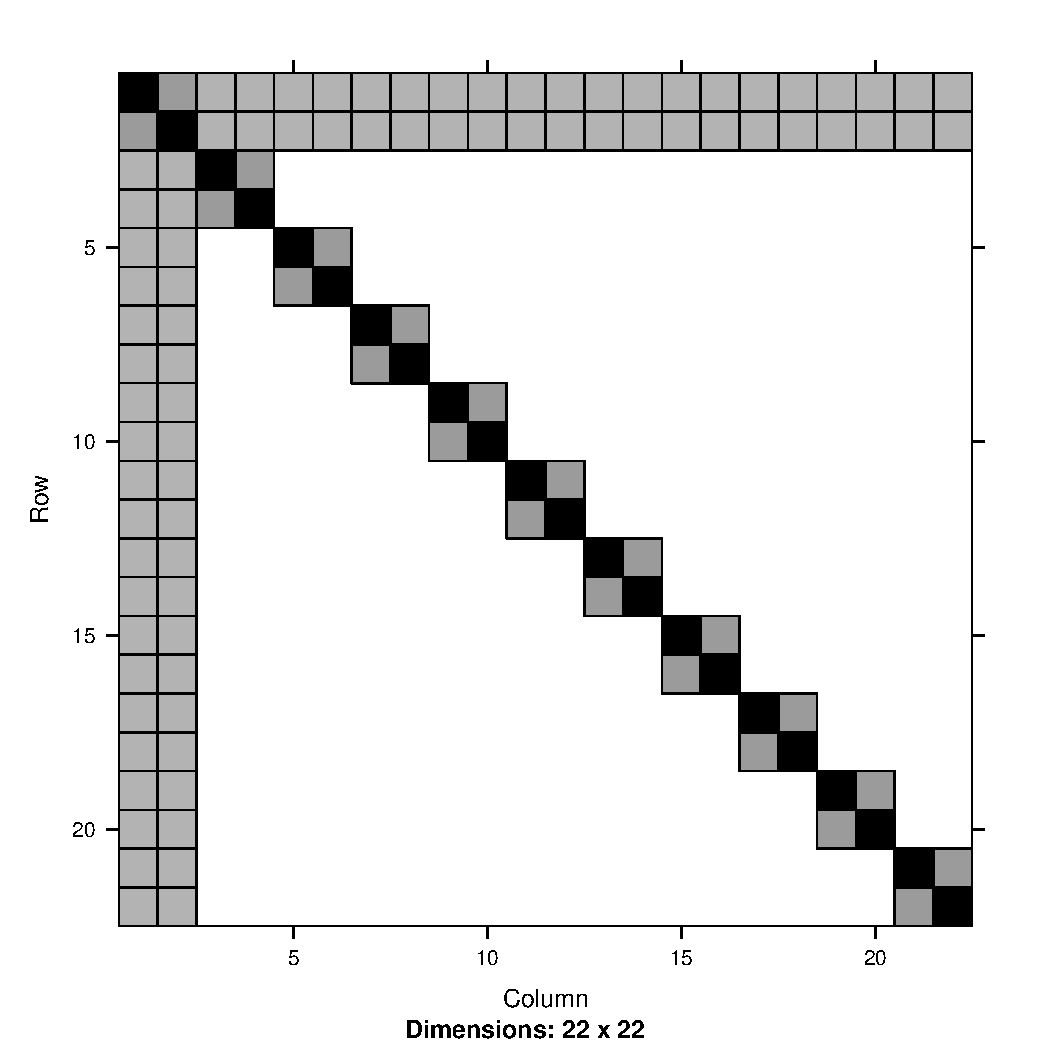
\includegraphics[width=0.45 \textwidth]{mX_mZ_mLambda.pdf}
	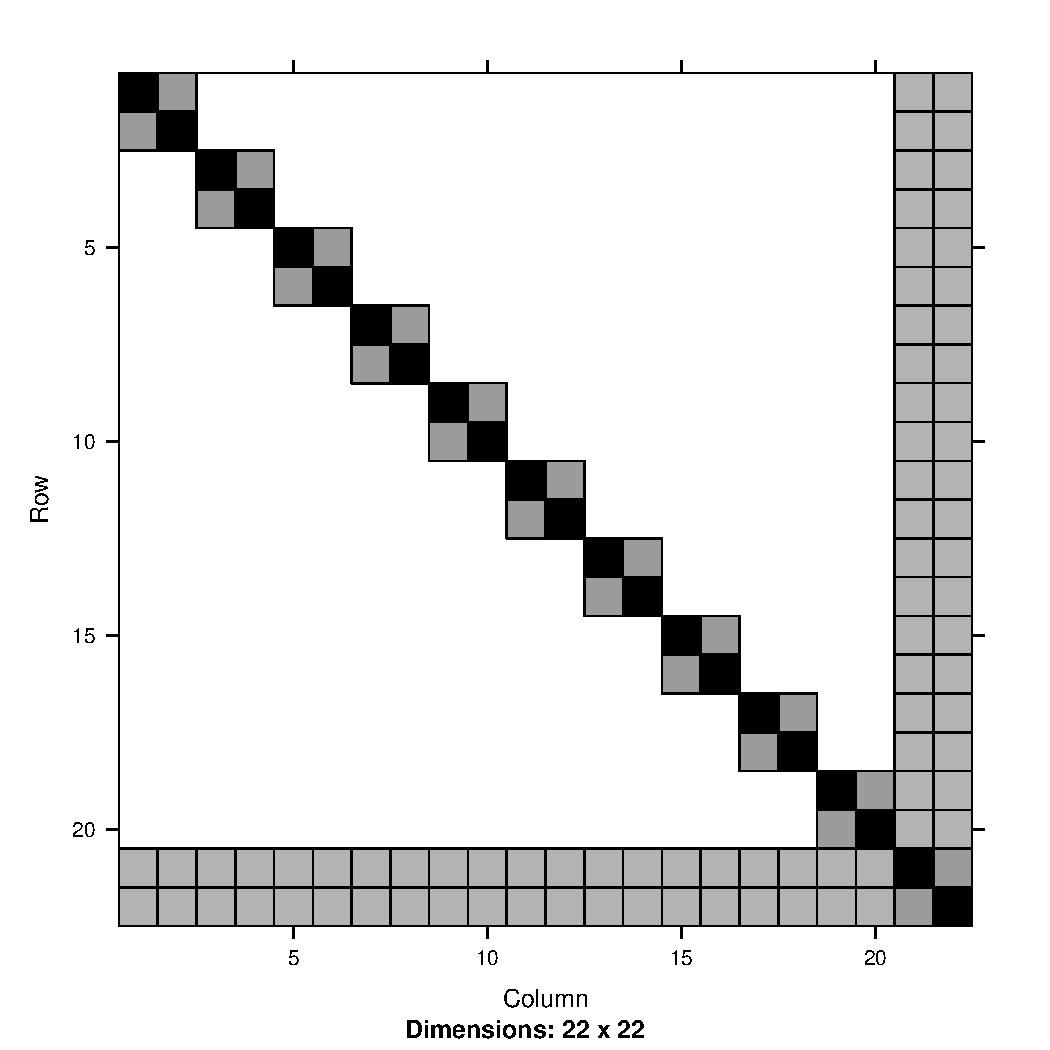
\includegraphics[width=0.45 \textwidth]{mZ_mX_mLambda.pdf}
	\caption{Inverse Covariance matrix of approximate posterior for $\vnu$ -- Fixed effects before random effects
						and random before fixed effects.}
	\label{fig:covfixedrandom}
\end{figure}
	
\begin{figure}[h!]
	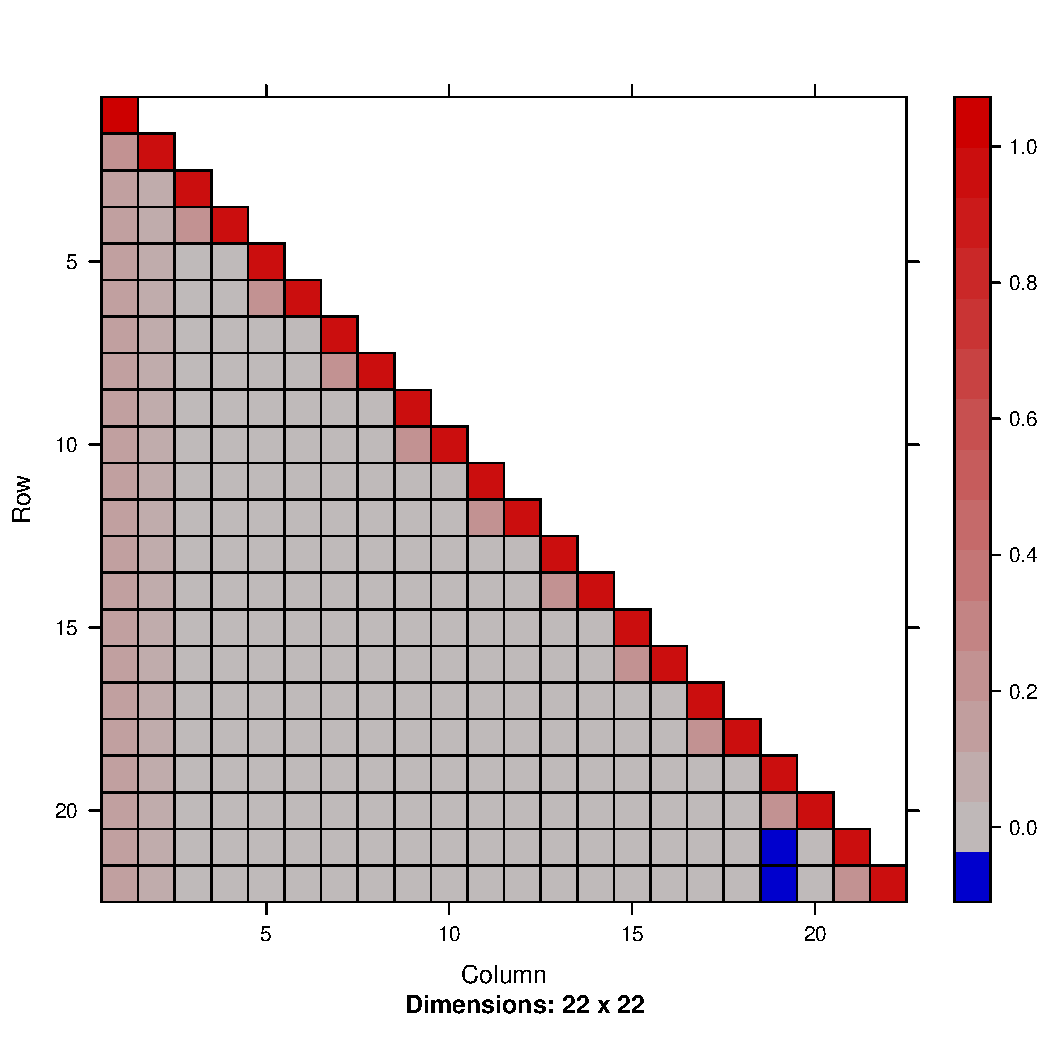
\includegraphics[width=0.45 \textwidth]{mX_mZ_cholesky.pdf}
	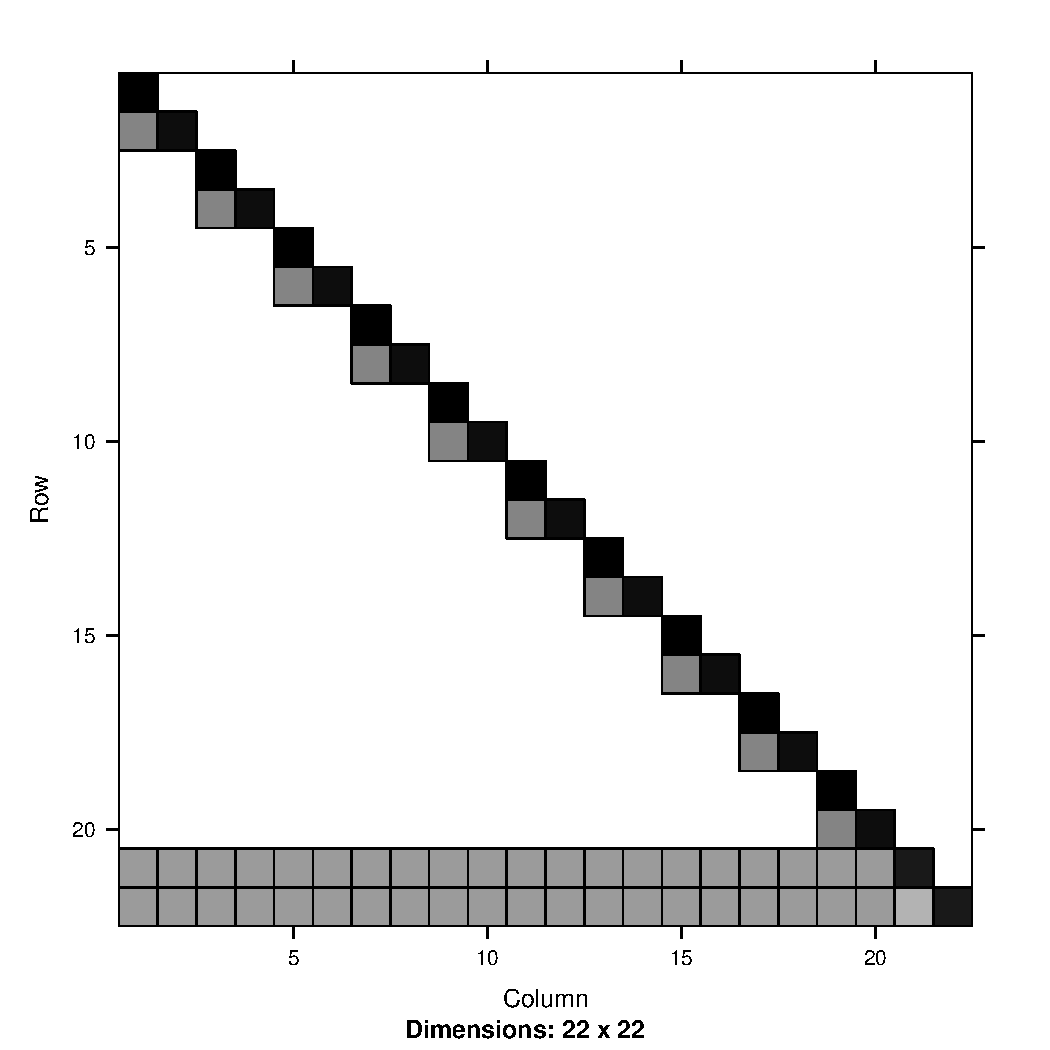
\includegraphics[width=0.45 \textwidth]{mZ_mX_cholesky.pdf}
	\caption{Cholesky factor of Inverse Covariance matrix of approximate posterior for $\vnu$ -- Fixed effects 
						before random effects and random before fixed effects.}
	\label{fig:cholfixedrandom}
\end{figure}

\subsection{Precision parameterisation}

We optimise over the space $(\vmu, \overline{\mR})$ as before, but now the elements of the Cholesky factor
are parameterised as
		
\begin{equation*}
\label{eq:cholesky_element_precision_param}
	\mR_{ij} =
	\begin{cases}
		\exp(-\overline{\mR}_{ij}), & i = j             \\
		\overline{\mR}_{ij},        & i > j             \\
		0,                          & \text{otherwise}.
	\end{cases}
\end{equation*}
	
\noindent This new choice of parameterisation allows us to calculate $\frac{1}{2} \text{diag}(\mC \mLambda
\mC^\top)$ by solving the linear systems $\mR \va = \mC_{i}, i=1, \ldots, n$ for   $\va$ and then calculating
$\va^\top\va$ where $\mC_{i} = $ the $i$th row of $\mC$, rather than calculating $\text{diag}(\mC \mLambda
\mC^\top)$ directly.
	
% TODO: We fixed this using safe-exp
The implementation of these algorithms was not without its' challenges, chiefly numerical issues encountered during testing and verification of the accuracy of the model fitting. Using the exponential function to parameterise the main diagonal coupled with L-BFGS-B's unconstrained line search and \texttt{optim()}'s lack of robustness to infinities lead to many overflow problems which may have been lessened or dealt with entirely by using a function with a less aggressive growth rate, such as an appropriate piecewise quadratic.
	
The main computational cost is the evaluation of the variational lower bound and its' derivatives. By
virtue of their dimension, the expressions involving $\mLambda$ dominate the computational cost. The key
term is $\frac{1}{2} \diag(\mC \mLambda \mC^\top)$. This can be naively calculate by ignoring the
symmetry in the expression and simply calculating the product $\mC \mLambda \mC^\top$, taking $2 n
\times (p + m b)^2$ floating point operations, and retaining the diagonal entries of the result. This is
obviously wasteful, as the off--diagonal entries of the resulting product that has just been computed
are immediately discarded.
	
By parameterising $\mLambda$ in terms of its' Cholesky factors and realising that
\begin{equation*}
	\mC \mLambda \mC^\top = \mC \mR \mR^\top \mC^\top
\end{equation*}
	
\noindent and that
\begin{equation*}
	\diag(\mC \mLambda \mC^\top)_{ii} = \mC_{i .} \mR \mR^\top \mC_{i .}^\top, 1 \leq i \leq n
\end{equation*}
	
\noindent we can calculate the products $\mC_{i .} \mR, 1 \leq i \leq n$, using $n \times \frac{1}{2}(p + m
b)(p + m b   + 1)$ floating point operations, and storing the results of the $i$th product in the $i$th
element of the   vector $\va$ and then calculate $\diag(\mC \mLambda \mC^\top) = \va^\top \va$.
	
Moreover, mixed models typically have sparse design matrices, allowing us to encode $\mR$ as a sparse matrix, and	further reduce   this depending on the model. For example, in the random intercept case, only the diagonals of the random effects block need to be non-zero, and hence the above expression can be calculated in
$\BigO(n)$ floating point operations.
	
% $\log |\mR|$ can be calculated using only $p + m b$ floating point operations, as $\mR$ is lower triangular.
	
For the precision parameterisation, we observe that in this parameterisation
\begin{equation*}
	\diag(\mC \mLambda \mC^\top)_{ii} = \mC_{i .} \mR^{-\top} \mR^{-1} \mC_{i .}^\top, 1 \leq i \leq n,
\end{equation*}
\noindent and so by solving $\mR \va = \mC_{i .}^\top$ for $\va$ for all $i$ at a cost of $n \times
\frac{1}{2} (p + m b) (p + m b + 1)$ floating point operations, and then calculating
\begin{equation*}
	\diag(\mC \mLambda \mC^\top)_{ii} = \va^\top \va, 1 \leq i \leq n,
\end{equation*}
\noindent we can then calculate $\diag(\mC \mLambda \mC^\top)$.
	
As above, by using our knowledge of the model being fit we can encode $\mR$ sparsely to decrease the required
computation still further. In the random intercept model case, the computational cost will drop to $n \times
\{m + \frac{1}{2} p (p + 1) + p \times m b\}$.
			
\subsubsection{Justification of Cholesky factor of the precision matrix as the parameterisation}
The Gaussian Variational Approximation is fit by maximising the Gaussian Variational Lower Bound, which is
parameterised by a mean vector $\vmu$ and a covariance matrix $\mLambda$. The most straightforward
parameterisation of $\vmu$ is the natural parameterisation. But the covariance matrix has many possible
parameterisations. Covariance matrices are positive semi-definite, and hence symmetric, so they have a unique
Cholesky factorisation. Parameterising the covariance matrix in terms of the Cholesky factor allows us to
represent the square covariance matrix using only a lower triangular matrix with half as many non-zero
elements. Thus the Cholesky factor is a convenient way to parameterise covariance matrices.

While the most obvious choice for parameterising the covariance matrix is simply the covariance matrix itself,
this is not the only available parameterisation. Another choice worth considering is parameterising the
covariance matrix using the Cholesky factor of the precision matrix.

The variational lower bound of a Gaussian Variational Approximation takes the form given in Equation
(\ref{eq:gva_lower_bound_precision_param2}).
\begin{equation}
\label{eq:gva_lower_bound_precision_param2}
\begin{array}{ll}
\log \underline{p}(\vy; \vmu, \mLambda) =& \vy^\top \mC \vmu - \vone^\top B(\mC \vmu, \text{diag}(\mC \mLambda \mC^\top)) + \vone^\top c(\vy) \\
&- \tfrac{1}{2} \vmu^\top \mSigma^{-1} \vmu - \tfrac{1}{2} \tr(\mSigma^{-1} \mLambda) \\
&+ \tfrac{1}{2} \log |\mLambda| - \tfrac{1}{2} \log |\mSigma| + \tfrac{d}{2}
\end{array}
\end{equation}

Let $\mOmega = \mLambda^{-1}$, the precision matrix. Then if we reparameterise the variational lower bound in
terms of $\mOmega$ we obtain the function in Equation (\ref{eq:gva_lower_bound_precision_param_omega}).
\begin{equation}
\label{eq:gva_lower_bound_precision_param_omega}
\begin{array}{ll}
F(\mOmega) =& \quad \vy^\top \mC \vmu - \vone^\top B(\mC \vmu, \text{diag}(\mC \mOmega^{-1} \mC^\top)) + \vone^\top c(\vy) \\
&- \tfrac{1}{2} \vmu^\top \mSigma^{-1} \vmu - \tfrac{1}{2} \tr(\mSigma^{-1} \mOmega^{-1}) \\
&- \tfrac{1}{2} \log |\mOmega| - \tfrac{1}{2} \log |\mSigma| + \tfrac{d}{2}
\end{array}
\end{equation}

When the variational lower bound is optimised, by the first-order optimality conditions, $\tfrac{\partial
F}{\partial \mOmega_{jk}} = \vzero$. Then using matrix calculus and the properties of the trace operator
\begin{equation*}
\begin{array}{ll}
\tfrac{\partial F}{\partial \mOmega_{jk}} &= -\tfrac{1}{2} \tr(\mOmega^{-1} \tfrac{\partial \mOmega}{\partial \mOmega_{jk}}) + \tfrac{1}{2} \tr(\mSigma^{-1} \mOmega^{-1} \tfrac{\partial \mOmega}{\partial \mOmega_{jk}} \mOmega^{-1}) \\
&\quad -\tfrac{1}{2} \tr\{\mC^\top \text{diag}(B^{(2)}(\mC \vmu, \text{diag}(\mC \mOmega^{-1} \mC^\top))) \mC \mOmega^{-1} \tfrac{\partial \mOmega}{\partial \mOmega_{jk}} \mOmega^{-1}\} \\
&=-\tfrac{1}{2} [ \tr(\mOmega^{-1} \mOmega \mOmega^{-1} \tfrac{\partial \mOmega}{\partial \mOmega_{jk}}) - \tr(\mSigma^{-1} \mOmega^{-1} \tfrac{\partial \mOmega}{\partial \mOmega_{jk}} \mOmega^{-1}) \\
&\quad + \tr\{\mOmega^{-1} \mC^\top \text{diag}(B^{(2)}(\mC \vmu, \text{diag}(\mC \mOmega^{-1} \mC^\top))) \mC \mOmega^{-1} \tfrac{\partial \mOmega}{\partial \mOmega_{jk}}\} ] \\
&= -\tfrac{1}{2} \tr[\mOmega^{-1}\{ \mOmega - \mC^\top \text{diag}(B^{(2)}(\mC \vmu, \text{diag}(\mC \mOmega^{-1} \mC^\top))) \mC - \mSigma^{-1} \} \mOmega^{-1} \tfrac{\partial \mOmega}{\partial \mOmega_{jk}}]
\end{array}
\end{equation*}

As $\mOmega^{-1} \ne \vzero$ and $\tfrac{\partial \mOmega}{\partial \mOmega_{jk}} \ne \vzero$, this implies
$\mOmega = \mC^\top \text{diag}(B^{(2)}) \mC + \mSigma^{-1}$. Thus the sparsity of $\mOmega$ depends on the
structure of $\mC$ and $\mSigma$, which depends on the model specified.

Another argument in favour of parameterising using the precision matrix is that the covariance matrix contains
the marginal covariances between the elements of $\vnu$, while the precision matrix contains the conditional
covariances betweenm those elements. In generalised linear mixed models, fixed and random effects are
conditionally independent, implying sparsity in the precision matrix although not necessarily in the
covariance matrix.

Still another advantage of this parameterisation is its' greater numerical accuracy.
Matrix multiplication and back substitution are both equally numerically accurate and stable --- see
\cite{Golub:1996:MC:248979} \S2.7.8 and \S3.1.2 or \cite{trefethen97} Lecture 17. Moreoever, as the precision
matrix will be sparse due to the specification of the mixed model/conditional independence, implying the
numerical accuracy of the inversion will be higher as there are fewer non-zero entries in the Cholesky factor
of the precision matrix than of the Cholesky factor of the covariance matrix. Thus parameterising the
variational lower bound in terms of the precision matrix will have the same or higher numerical accuracy than
parameterising in terms of the covariance matrix.

\section{Numerical results}
\label{sec:results}
		
The accuracy of each model fitting algorithms presented in Section \ref{sec:gaussian} was assessed by
comparing the approximating distribution of each parameter with the posterior distribution of Monte Carlo
Markov Chain samples of that parameter. 1 million Monte Carlo Markov Chain samples were generated using
\texttt{RStan}, as described in \cite{Carpenter2016} and \cite{StanDevelopmentTeam2016}. The accuracy of
examples of random intercept, random slope and spline models were evaluated using this method.
		
\subsection{Simulated data}
		
For each of these simulations, the model is as presented in Section \ref{sec:model}. Several common
application scenarios were simulated and their accuracy evaluated. A random intercept model was simulated with
$\vbeta = (2, 1)^\top$, $\rho = 0.5$, $m = 20$, $n_i = 10$ and $b = 1$. The results are presented in Table
\ref{tab:accuracy_int}. A random slope model was simulated with $\vbeta = (2, 1)^\top$, $\rho = 0.5$, $m =
20$, $n_i = 10$ and $b = 2$. The results are presented in Table \ref{tab:accuracy_slope}. Spline model was fit
to a data set generated from the function $3 + 3 \sin{(\pi x)}$ on the interval $[-1, 1]$. The resulting model
fits are presented in Figure \ref{fig:spline}.
		
To assess the speed of each approach, a test case was constructed of a random slope model with $m=50$
groups, each containing $n_i = 100$ individuals. A model was then fit to this data set ten times using
each algorithm, and the results averaged. They are presented in Table \ref{tab:application_slope_speed}.

\begin{table}
	\begin{tabular}{|l|rr|}
		\hline
		Algorithm & Mean (seconds) & Standard deviation (seconds) \\
		\hline
		Laplace's method & $0.37$ & $0.07$ \\
		GVA covariance parameterisation & $2.04$ & $1.24$ \\
		% Why is this slower?
		GVA inverse parameterisation & $0.38$ & $0.66$ \\
		GVA fixed point & $0.05$ & $0.07$ \\
		\hline
	\end{tabular}
	\caption{Table of results - Speed}
	\label{tab:application_slope_speed}
\end{table}

% The stability of the algorithms was confirmed by running them on 10,000 different data sets that were randomly
% generated after having initialised the random number generator with different seeds.
		
Median accuracy of the algorithms was assessed by running them on 100 randomly generated data sets. The	results are presented in Figure \ref{fig:median_accuracy_intercept} and Figure
\ref{fig:median_accuracy_slope}.
		
% Figure: Median accuracy graph intercept
\begin{figure}[h]
	\begin{center}
		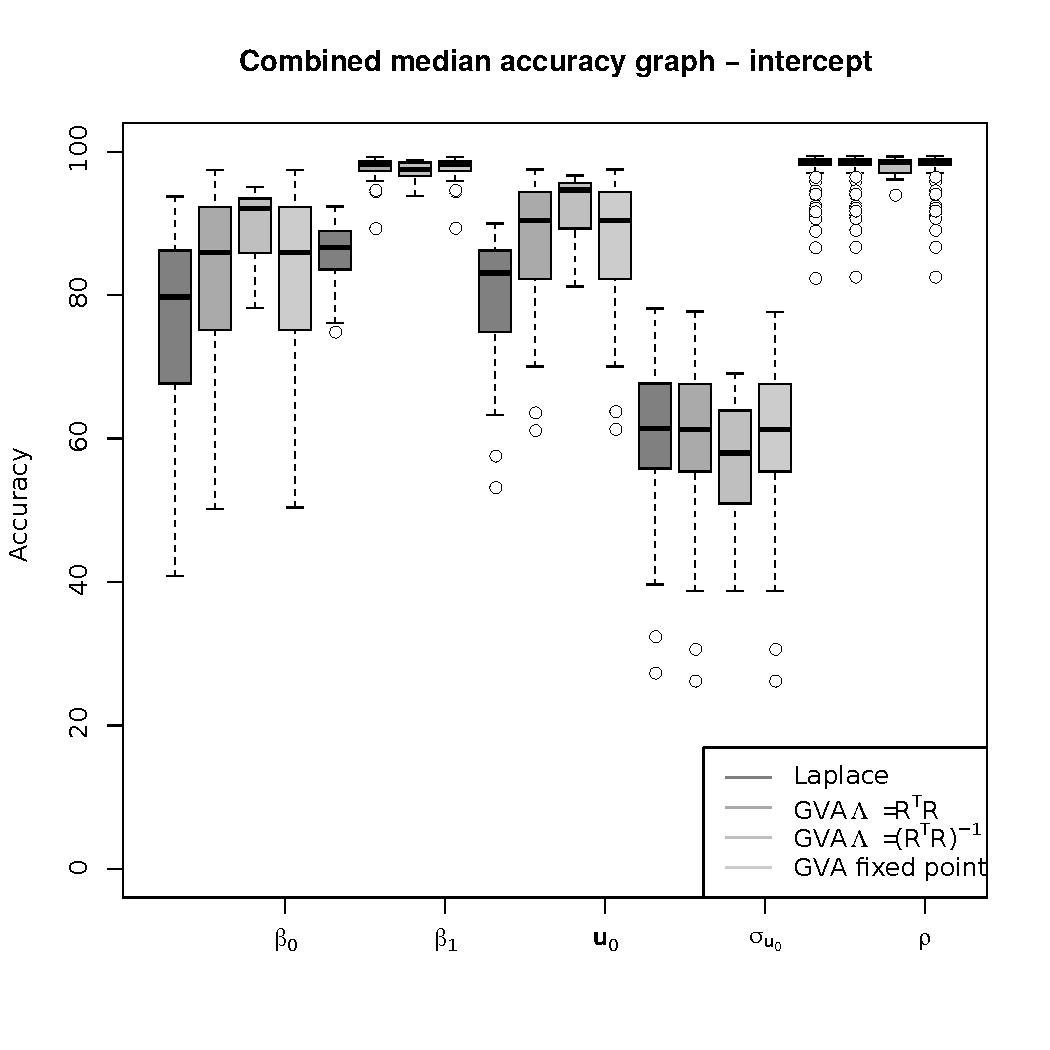
\includegraphics[width=0.95\textwidth]{code/results/median_accuracy_combined_intercept.pdf}
		\caption{Boxplots of accuracies of the parameter estimates for a random intercept model after 100 repeated
							runs on simulated data. We see that the accuracy of the parameter estimates is quite stable,
							and the median accuracies are high.}
		\label{fig:median_accuracy_intercept}
	\end{center}
\end{figure}
		
% Figure: Median accuracy graph slope
\begin{figure}[h]
	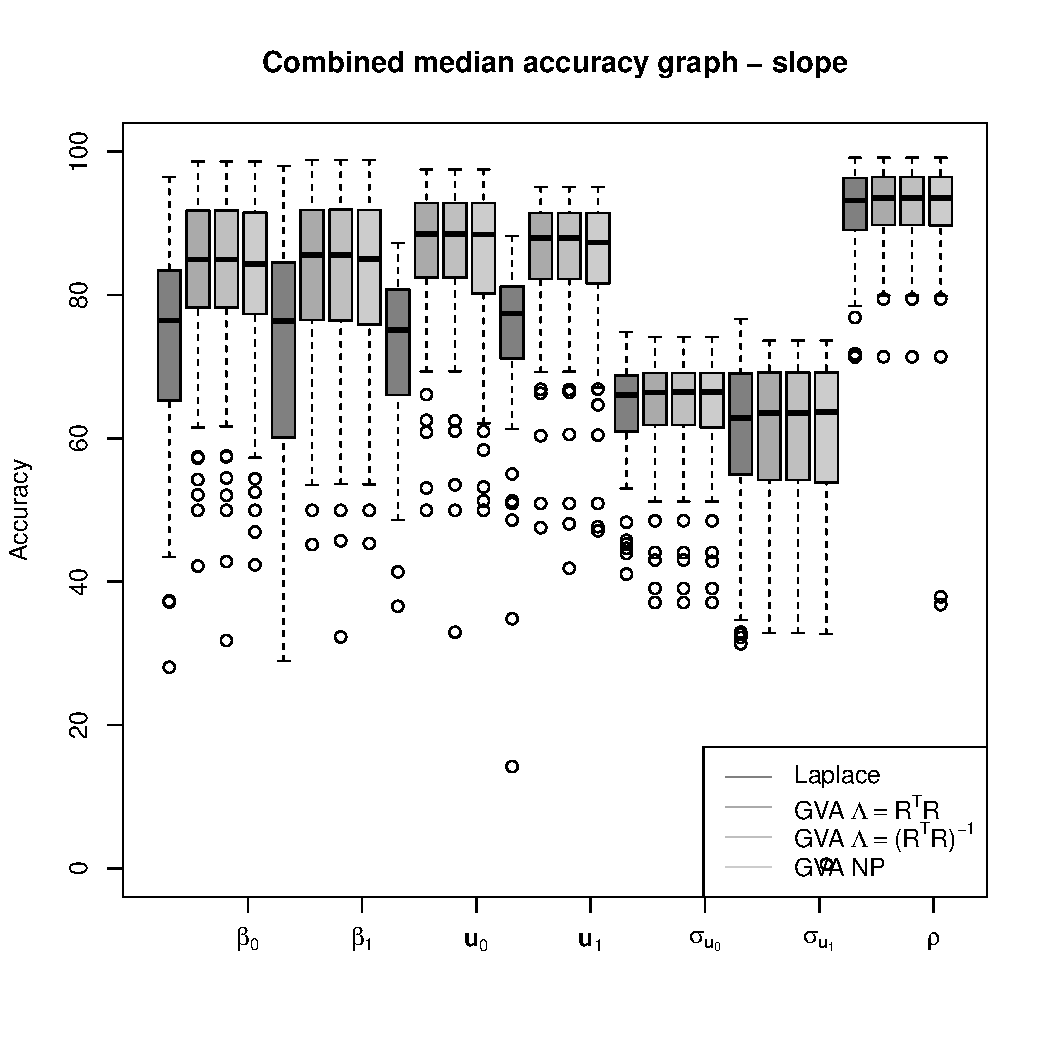
\includegraphics[width=0.95\textwidth]{code/results/median_accuracy_combined_slope.pdf}
	\caption{Boxplots of accuracies of the parameter estimates for a random slope model after 100 repeated
							runs on simulated data. We see that the accuracy of the parameter estimates is quite stable,
							and the median accuracies are high.}
	\label{fig:median_accuracy_slope}
\end{figure}
		
% Table of accuracy results - intercept model
\begin{table}
	\begin{tabular}{|l|rrrr|}
		\hline
		                   & Laplace's Method & GVA $(\mLambda = \mR \mR^\top)$ & GVA NP $(\mLambda = (\mR \mR^\top)^{-1})$ & GVA FP \\
		\hline
		$\vbeta_1$         & $85\%$           & $90\%$                          & $91\%$                                    & $90\%$ \\ 
		$\vbeta_2$         & $76\%$           & $98\%$                          & $99\%$                                    & $99\%$ \\ 
		Mean of $\vu$      & $81\%$           & $94\%$                          & $94\%$                                    & $94\%$ \\
		$\sigma^2_{\vu_1}$ & $66\%$           & $66\%$                          & $66\%$                                    & $66\%$ \\ 
		$\rho$             & $99\%$           & $99\%$                          & $99\%$                                    & $99\%$ \\ 
		\hline
	\end{tabular}
	\caption{Table of accuracy - Random intercept model}
	\label{tab:accuracy_int}
\end{table}
		
\begin{table}
	\begin{tabular}{|l|rrrr|}
		\hline
		                   & Laplace's Method & GVA $(\mLambda = \mR \mR^\top)$ & GVA $(\mLambda = (\mR \mR^\top)^{-1})$ & GVA FP \\
		\hline
		$\vbeta_1$         & $67\%$             & $88\%$                            & $88\%$                                   & $88\%$   \\
		$\vbeta_2$         & $70\%$             & $89\%$                            & $88\%$                                   & $89\%$   \\
		Mean of $\vu$      & $70\%$             & $91\%$                            & $91\%$                                   & $91\%$   \\
		$\sigma^2_{\vu_1}$ & $71\%$             & $73\%$                            & $73\%$                                   & $73\%$   \\
		$\sigma^2_{\vu_2}$ & $68\%$             & $69\%$                            & $69\%$                                   & $69\%$   \\
		$\rho$             & $91\%$             & $90\%$                            & $90\%$                                   & $90\%$   \\
		\hline
	\end{tabular}
	\caption{Table of accuracy - Random slope model}
	\label{tab:accuracy_slope}
\end{table}
		
% \begin{table}
% \caption{Table of accuracy - Splines}
% \label{tab:accuracy_spline}
% \begin{tabular}{|l|l|}
% \hline
% Approximation & Accuracy \\
% \hline
% Laplace's Method & 0.969 \\
% GVA & 0.969 \\
% GVA NP & 0.969 \\
% GVA NR & 0.969 \\
% \hline
% \end{tabular}
% \end{table}
		
\begin{figure}[h]
	\label{fig:spline}
	\caption{Comparison of VB and MCMC spline fits with the true function}
	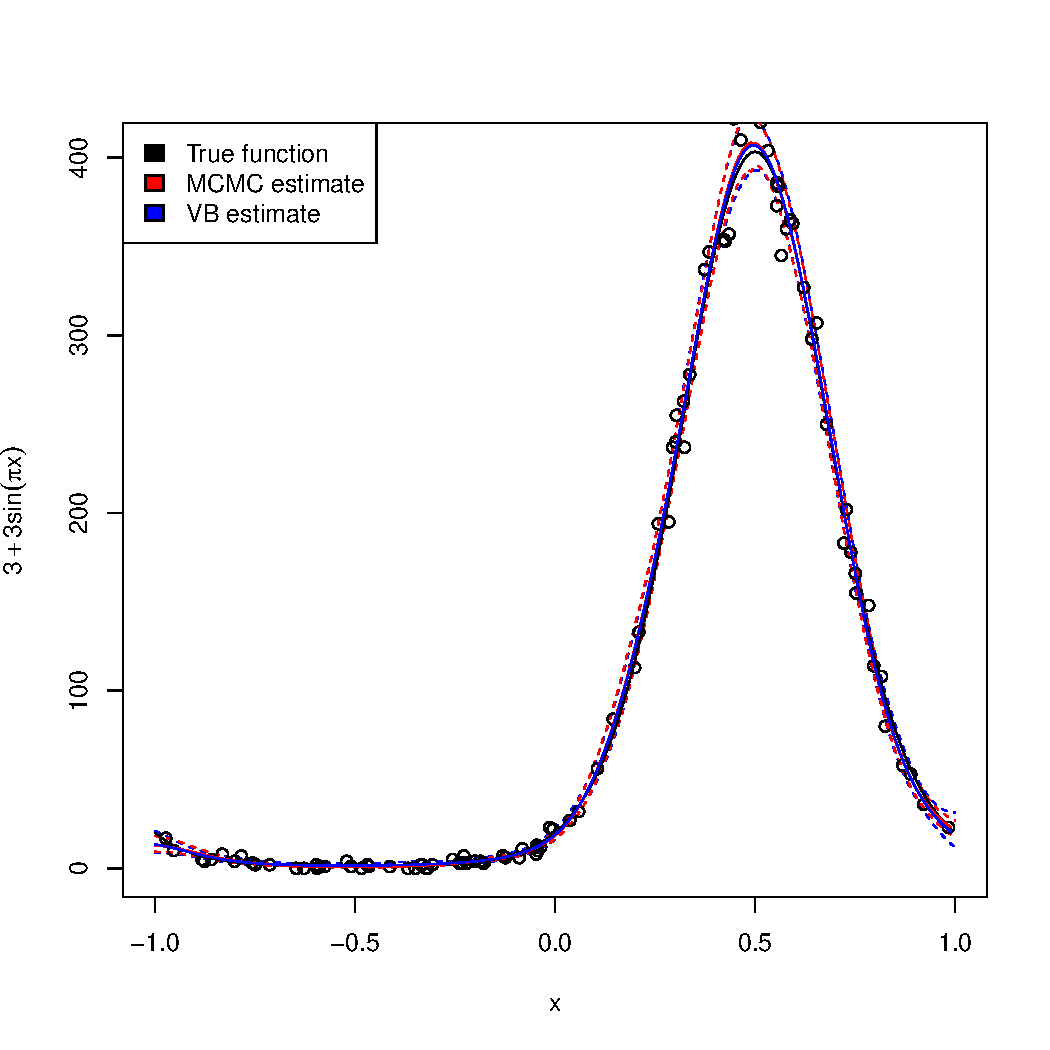
\includegraphics[width=0.95 \textwidth]{code/results/accuracy_plots_spline_gva2.pdf}
\end{figure}
		
% Graphs - exactly what sort of graphs do we need?
% Median accuracy
% Increase in lower bound
% MCMC posterior, with approximating posterior for at least one or two of the
% key parameters, such as, say, vbeta[2]
		
\subsection{Numerical stability of the parameterisation}

In the process of performing numerical experiments, we discovered that our model fitting software was
prone to numeric overflow due to the log link in our model and the exponentiation of the diagonals of
the Cholesky factors in the covariance parameterisation of the Gaussian Variational Approximation of
$\vnu$.

We dealt with this difficulty by developing a 'safe exponential' parameterisation for the diagonals of
the Cholesky factors. The parameterisation is exponential up to a threshold $t$, and then quadratic
beyond that threshold.

The stability of this scheme was tested by calculating the accuracy of the approximations fit with a
range of safe exponential thresholds, the results of which are presented in Figure
\ref{fig:stability_accuracy}. The variational approximation was found to be stable, with the accuracy
largely insensitive to the choice of threshold.

\begin{figure}[h]
	\includegraphics[width=0.95 \textwidth]{code/stability_intercept.pdf}
	\label{fig:stability_accuracy}
	\caption{Accuracy of approximation of parameters versus the safe exponential threshold}
\end{figure}

We repeated our numerical experiments with the new parameterisation, varying the threshold within
reasonable bounds and found that the numerical experiments no longer resulted in overflow, and that the
numerical accuracy of the approximation was still very good.

The stability of the GVA algorithm with the parameterisation $\mLambda = (\mR^\top \mR)^{-1}$ depends on
the threshold chosen for the safe exponential function. When the threshold is set to $2$, the algorithm
is stable for all starting points within the grid except $6$. When the threshold is set to $\infty$,
equivalent to using the naive $\exp$ parameterisation, the algorithm encounters numerical errors for
every starting point on the  grid.
	
\subsection{Stability of the GVA precision parameterisation algorithm for different starting points}
		
The numerical stability of each fitting algorithm in Section \ref{sec:gaussian} was assessed by
initialising each algorithm from a range of different starting points. Errors due to numerical
instability and the fitted $\vmu$ were recorded for each starting point.
		
A data set of 100 individuals in ten groups ($m=10$) was generated from a model with a fixed intercept
and slope, and a random intercept. $\vmu$ was initialised from a grid of points on the interval $[-4.5,
5]$ for intercept and slope, spaced $0.1$ apart. The error counts are presented in Table
\ref{tab:stability_results}. Plots of the starting locations which resulted in numerical errors when the
fitting algorithm was run are presented in \ref{fig:stability_locations_gva}.
		
\begin{table}
	\begin{tabular}{|l|r|}
		\hline
		Algorithm                            & Error count \\
		\hline
		Laplace's algorithm                  & $12$          \\
		GVA $\mLambda = \mR^\top \mR$        & $1306$       \\
		GVA $\mLambda = (\mR^\top \mR)^{-1}$ & $6$           \\
		GVA NR fixed point                   & $992$         \\
		\hline
	\end{tabular}
	\caption{Count of numerical errors for each algorithm during stability tests}
	\label{tab:stability_results}
\end{table}

The GVA algorithm with the $\mLambda = (\mR \mR^\top)^{-1}$ parameterisation was less prone to
instability due to starting point when the safe exponential parameterisation was used then when it was
not used, as can be seen from Figure \ref{fig:stability_locations_gva}. % FIXME: Add error counts
		
\begin{figure}[h]
	\includegraphics[width=0.45 \textwidth]{code/safe_exp_stability.pdf}
	\includegraphics[width=0.45 \textwidth]{code/no_safe_exp_stability.pdf}
	\label{fig:stability_locations_gva}
	\caption{Starting locations which caused the GVA fitting algorithm to fail with numeric errors. The true model had fixed parameters $\vbeta = (2, 1)^\top$ and random intercepts. There were ten groups in the hierarchical model each	with ten individuals $(m=10, n_i=10)$. In the left figure the starting points which lead to numeric errors when the safe exponential was used are shown, while in the right figure the starting points which lead to numeric errors when the safe exponential was not used are plotted.}
\end{figure}

\subsection{Stability of the GVA fixed point algorithm for different starting points}
The naive fixed point algorithm was extremely unstable for many starting points, as can be seen from
Figure \ref{fig:stability_locations_nr}. The variant of the algorithm which checked whether the
inversion of the $\mLambda_{\vu \vu}$ block of $\mLambda$ was performed successfully was much more
stable, and did not suffer from any numeric errors at all over the range of starting points we tested.
The algorithm is able to abort safely, and allow the Variational Bayes algorithm to update the other
parameters before trying to fit the Gaussian component of the model again until the correct parameters
are accurately estimated.

\begin{figure}[h!]
	\includegraphics[width=0.95 \textwidth]{code/local_solutions_gva_nr_error_locations_no_protections.pdf}
	\label{fig:stability_locations_nr}
	\caption{Starting locations which caused the NR fitting algorithm to fail with numeric errors. The true model had fixed parameters $\vbeta = (2, 1)^\top$ and random intercepts. There were ten groups in the
	hierarchical model each	with ten individuals $(m=10, n_i=10)$}
\end{figure}

\section{Application}
We now present numerical results for the application of our model fitting algorithms to several real-world
data sets.

\label{sec:application}

\subsection{Poisson example without zero-inflated component -- Police stops}
\label{sec:police_stops}
The data set used for this example was the police stop example from Chapter 15 of \cite{Gelman2007}.
The model fit was
$$
	\vy_{ep}        \sim \text{Poisson}(n_{ep} e^\vnu)
$$
where $\vnu = {\beta_0 + \beta_e \text{ethnicity}_e + \alpha_{c} \text{crime} + \vu_p}$, with priors
\begin{align*}
	\valpha				& \sim \N(0, \sigma_\valpha^2),	\\
	\vbeta        & \sim \N(0, \sigma_\vbeta^2), \text{ and }\\
	\vu_p         & \sim \N(0, \sigma_\vu^2)
\end{align*}
where $p$ is the $p$-th precinct, and $e$ is the $e$-th ethnicity (blacks, hispanics or whites), and $c$ is
the $c$-th category of crime (violent crimes, weapons crimes, propery crimes or drug crimes). The random
intercepts $u_p$ allow for variation in the base rates of stops across precincts, the co-efficients $\beta_j$
measure the effect of ethnicity on the rate of police stops and the co-efficients $\alpha_k$ measure the
effect of each type of crime on the rate. The model finds the relationship between the number of police stops
in each precinct and  ethnicity for each type of crime.

The model was fit using the GVA algorithm with the $\mLambda = (\mR^\top \mR)^{-1}$ parameterisation, using
the prior $a_\rho = 3$, $b_\rho = 1$ on $\rho$. Accuracy of the approximation was assessed by comparing the
fitted distribution for each parameter to a kernel density estimate of the parameter's distribution from 1
million samples from the equivalent model fitted using Stan. The results are presented in Table
\ref{tab:application_police_stops}. Figure \ref{fig:police_stops}

\begin{figure}[h]
\includegraphics[width=0.95 \textwidth]{code/results/accuracy_plots_application2_GVA_inv_par-highlights-nup.pdf}
\caption{Accuracy of parameter estimates for police stops}
\label{fig:police_stops}
\end{figure}

% Table of results
\begin{table}
	\begin{tabular}{|l|rrrr|}
		\hline
		Covariate                     & Posterior Mean & Lower 95\% CI & Upper 95\% CI & Accuracy \\
		\hline
		Intercept [African-Americans] & $4.04$          & $3.98$           & $4.07$          & 82\%   \\
		$\beta_2$ [hispanics]         & $-0.45$         & $-0.46$          & $-0.43$         & 98\%   \\
		$\beta_3$ [whites]            & $-1.38$         & $-1.40$          & $-1.37$         & 99\%   \\
		$\alpha_1$ [weapons crimes]   & $0.58$          & $0.57$           & $0.59$          & 89\%   \\
		$\alpha_2$ [property crimes]  & $-0.19$         & $-0.21$          & $-0.17$         & 92\%   \\
		$\alpha_3$ [drug crimes]      & $-0.75$        & $-0.77$          & $-0.73$         & 95\%   \\
		Random intercept              & $1.32$         & $-0.19$         & $2.20$         & 87\%   \\
		$\sigma^2_{\vu}$              & $8.57$          & $1.02$           & $24.35$         & 49\%     \\
		\hline
	\end{tabular}
	\caption{Table of results - Police stops}
	\label{tab:application_police_stops}
\end{table}

% Table of speeds
\begin{table}
	\begin{tabular}{|ll|}
		\hline
		Algorithm & Time  in seconds \\
		\hline
		Laplace & $0.24$ \\
		GVA covariance parameterisation & $6.02$ \\
		GVA inverse paramaterisation & $3.92$ \\
		GVA fixed point & $0.18$ \\
		\hline
	\end{tabular}
	\caption{Table of speeds - Police stops}
	\label{tab:police_stop_speeds}
\end{table}

% TODO: You need to describe the data set and the model.
\subsection{Zero--inflated example -- Cockroaches in apartments}
\label{sec:cockroaches}
The model described in this section was fit  to the cockroach data set from Section 6.7 of
\cite{Gelman2007}, taken from a study on the effect of integrated pest management in controlling
cockroach levels in urban apartments. The data set contains data on 160 treatment and 104 control
apartments, along with the response $y_i$ in each apartment of the number of cockroaches caught in a set
of traps. The apartments had the traps deployed for different numbers of days, referred to as trap days,
which was handled by using a log offset \cite{Agresti2002}. The predictors in the data set included the
pre-treatment roach level, a treatment indicator, the time of the observation and an indicator for
whether the apartment is in a senior building restricted to the elderly.
		
In the example application presented in this paper, the zero component represents an apartment completely free of roaches, while the non-zero component represents an apartment where roaches have been able to live and reproduce, possibly in spite of pest control treatment aimed at preventing them from doing so.

The model fit was
$$
	y_i = \begin{cases}
	0, \phantom{-} \text{if} \phantom{-} R_i = 0, \\
	\text{Poisson}(e^{\mX_i \vbeta + \mZ_i \vu}), \phantom{-} \text{if} \phantom{-} R_i = 1
	\end{cases}
$$
with priors
\begin{align*}
	R_i &\sim \text{Bernoulli}(\rho), \\
	\rho &\sim \text{Beta}(a, b), \\
	\vbeta &\sim \text{N}(\vzero, \sigma^2_\vbeta \mI), \\
	\vu &\sim \text{N}(\vzero, \mSigma) \text{ and } \\
	\mSigma &\sim \text{Inverse-Wishart}(\mPsi, v)
\end{align*}
with prior parameters $a = 1$, $b = 1$, $\sigma^2_\vbeta = 10^5$, $\mPsi = 10^{-5} \mI$ and $v = 2$.
These priors were chosen to be vaguely informative for the variance components and a uniform prior for
the zero-inflation proportion latent variable $\rho$. The fixed effects covariates included in the
model were time in days and time in days $\times$ pest control treatment. A random intercept to account
for variation between the apartment buildings was included.
		
The GVA algorithm with the $\mLambda = (\mR^\top \mR)^{-1}$ parameterisation was used to fit a random
intercept model to the Roaches data set provided \cite{Gelman2007}. The fitted co-efficients and accuracy
results are presented in Table \ref{tab:application_roaches}.
		
%       lci  uci
% 1  3.179 3.157 3.201
% 2 -0.046 -0.053 -0.039
% 3 -0.420 -0.434 -0.406
% 1 -0.976 -1.015 -0.936
% 2 -0.309 -0.323 -0.295
% 3 -0.947 -0.963 -0.930
% 4 -2.129 -2.384 -1.874
% 5 -3.230 -3.490 -2.970
% 6 -3.099 -3.404 -2.794
% 7 -1.290 -1.326 -1.255
% 8 -0.956 -0.991 -0.921
% 9 -2.404 -2.600 -2.209
% 10 -1.076 -1.123 -1.029
% 11 -1.079 -1.107 -1.052
% 12 -1.681 -1.737 -1.624
		
%> round(cbind(fit1$vmu, lci, uci), 3)
% fit1$a_rho
% [1] 377.2375
% > fit1$b_rho
% [1] 152.7625
		
\begin{table}
	\begin{tabular}{|l|rrrr|}
		\hline
		Covariate          & Posterior Mean & Lower 95\% CI & Upper 95\% CI & Accuracy \\
		\hline
		Intercept          & $3.42$						& $3.2$ 					& $3.65$          & $95\%$     \\
		Time               & $-0.14$        & $-0.05$       & $-0.02$       & $96\%$     \\
		Time:Treatment     & $-0.31$        & $-0.43$       & $-0.14$       & $96\%$     \\
		Random intercept   & $-1.60$        & $-1.71$       & $-1.49$       & $90\%$     \\
		$\sigma^2_{\vu_1}$ & $3.29$           & $2.02$          & $8.48$          & $63\%$     \\
		$\rho$             & $0.51$           & $0.50$          & $0.55$          & $62\%$     \\
		\hline
	\end{tabular}
	\caption{The posterior means, 95\% credible intervals and accuracy of the fixed and random
						effects, $\sigma_{\vu_1}^2$ and $\rho$ for the Roach model.}
	\label{tab:application_roaches}
\end{table}

\begin{table}
	\begin{tabular}{|lr|}
	\hline
	Algorithm & Time in seconds \\
	\hline
	Laplace & $0.49$ \\
	GVA & $1.08$ \\
	GVA inv. param & $0.81$ \\
	GVA fixed point & $0.11$ \\
	\hline
	\end{tabular}
	\label{tab:application_roaches_runtime}
	\caption{The runtimes in seconds for fitting algorithms when fitting the roach model.}
\end{table}
		
\begin{figure}[h]
	\centering
	% \includepdf[width=75mm,height=75mm,pages={1,2,3,16},nup=2x2]{code/results/accuracy_plots_application_GVA2.pdf}
	\begin{tabular}{@{}c@{\hspace{.5cm}}c@{}}
	\includegraphics[width=0.95 \textwidth]{code/results/accuracy_plots_application_GVA_inv_param-highlights-nup.pdf}
	\end{tabular}
	\caption{Accuracy graphs for roach model}
	\label{fig:accuracy_roach}
\end{figure}
		
\subsection{Example - Biochemists}
\label{sec:biochemists}
The model described in this section was fit to the biochemistry data set analysed by
\cite{Long1990}. The sample was taken from 915 biochemistry graduate students. The outcome
$\vy_i$ is the number of articles published in the last three years of the PhD. The covariates were the
gender of the student, coded $1$ for female and $0$ for male, the marital status of the student ($1$ for
married, $0$ for unmarried), the number of children under age six and the prestige of the PhD program.

In this example application, the zero component represents the number of biochemists who did not publish
any articles during the last three years of their PhD. Examination of the data reveals that this number
is higher than would be expected if the data followed a purely Poisson distribution -- 30\% of
biochemistry graduate students published no articles in their final years whereas a Poisson distribution
would predict only 18\%. This justifies our choice of model.

The model fit was
$$
	y_i = \begin{cases}
	\begin{array}{ll}
	0, & \text{if} R_i = 0, \\
	\text{Poisson}(e^\vnu), & \text{if} \phantom{-} R_i = 1,
	\end{array}
	\end{cases}
$$

\noindent where $\vnu = \vbeta_1 + \vbeta_2 \text{female} + \vbeta_3 \text{married} + \vbeta_4 \text{children under age 6} + \vbeta_5 \text{PhD}$, with priors
\begin{align*}
R_i &\sim \text{Bernoulli}(\rho), \\
\rho &\sim \text{Beta}(A, B) \text { and } \\
\vbeta &\sim \text{N}(0, \sigma_\vbeta^2 \mI)
\end{align*}

\noindent with $A=1$, $B=1$ and $\sigma_\vbeta^2 = 10,000$. The model was fit using the GVA inverse parameterisation algorithm. The resulting model fit is presented in Table \ref{tab:biochemists_results}
The accuracy of the parameter estimates is presented in Figure
\ref{fig:biochemists}. As this is a fixed effects model with a large number of samples relative to the
number of parameters being fit, we are able to estimate all of the parameters with great accuracy.

\begin{figure}[h]
\includegraphics[width=0.95 \textwidth]{code/results/accuracy_plots_application_biochemists_GVA_inv_param-nup.pdf}
\label{fig:biochemists}
\caption{Accuracy of the approximations of the parameters fit to the biochemists data}
\end{figure}

\begin{table}
	\begin{tabular}{|l|rrrr|}
		\hline
		Covariate          & Posterior Mean & Lower 95\% CI & Upper 95\% CI & Accuracy \\
		\hline
		Intercept & $0.86$ & $0.65$ & $1.06$ &  $95\%$ \\
		Female & $-0.18$ & $-0.29$ & $-0.08$ &  $95\%$ \\
		Married & $0.06$ & $-0.05$ & $0.18$ & $96\%$ \\
		Children under age 6 & $-0.08$ & $-0.15$ & $-0.01$ & $97\%$ \\
		PhD & $0.03$ & $-0.02$ & $-0.01$ & $97\%$ \\
		\hline
	\end{tabular}			
	\label{tab:biochemists_results}
	\caption{The posterior means, 95\% credible intervals and accuracy of the fixed effects for the 
						Biochemists model.}
\end{table}

\begin{table}
	\begin{tabular}{|l|r|}
	\hline
	Algorithm & Time in seconds \\
	\hline
	Laplace & $1.01$ \\
	GVA & $0.96$ \\
	GVA inv. param & $0.68$ \\
	GVA fixed point & $0.41$ \\
	\hline
	\end{tabular}
	\label{tab:biochemists_runtime}
	\caption{The runtimes in seconds for fitting algoritms when fitting the Biochemists model.}
\end{table}

\subsection{Example - Owls}
\label{sec:owls}
The model described in this section was fit to the Owls data set from taken from \cite{zuur_mixed_2009}.
The sample was 599 observations of owls grouped across 25 nests.The fixed covariates
fit in the model were food treatment (Deprived or Satiated) and arrival time, a continuous covariate.
The variation between the 25 different nests sampled from was modelled by a random intercept
$\vu$.

The model fit was
$$
	y_i = \begin{cases}
	\begin{array}{ll}
	0, & \text{if} R_i = 0, \\
	\text{Poisson}(e^\vnu), & \text{if} \phantom{-} R_i = 1,
	\end{array}
	\end{cases}
$$
where $\vnu = {\vbeta_2 \text{Food Treatment = Satiated} + \vbeta_3 \text{Arrival Time} + \vu_n}$ and $n$ is the $n$-th nest, with priors
\begin{align*}
R_i &\sim \text{Bernoulli}(\rho), \\
\rho &\sim \text{Beta}(A, B), \\
\vbeta &\sim \text{N}(\vzero, \sigma_\vbeta^2 \mI), \\
\vu &\sim \text{N}(0, \sigma_\vu^2) \text { and } \\
\sigma_\vu^2 &\sim \text{Inverse-Gamma}(s, t).
\end{align*}
where $\sigma_\vbeta^2=10,000$, $A=1$, $B=1$, $s=10^{-2}$ and $r=10^{-2}$.

The model was fit using the GVA inverse parameterisation algorithm. The accuracy of the parameter
estimates is shown in Figure \ref{fig:owls}. The variance component
The runtime of the algorithms is shown in Table
\ref{tab:owls_times}. We draw attention to the difference in run-times between the covariance and
inverse parameterisations. The inverse parameterisation is significantly faster -- $1.88$ seconds versus
$5.66$ seconds for the covariance parameterisation.

\begin{figure}[h]
	\includegraphics[width=0.95 \textwidth]{code/results/accuracy_plots_application_owls_GVA_inv_param-highlights-nup.pdf}
	\caption{Accuracy of the approximations of the parameters fit to the Owls data}
	\label{fig:owls}
\end{figure}

\begin{table}
	\begin{tabular}{|l|rrrr|}
		\hline
		Covariate          & Posterior Mean & Lower 95\% CI & Upper 95\% CI & Accuracy \\
		\hline
		Satiated & $-0.22$ & $-0.21$ & $-0.21$ & $97\%$ \\
		Arrival Time & $-0.07$ & $-0.07$ & $-0.07$ & $73\%$ \\
		Random intercept (nest) & $0.34$ & $-5.28$ & $5.96$ & $84\%$ \\
		$\sigma_{\vu_1}^2$ & $7.90$ & $3.21$ & $468.12$ & $94\%$ \\
		$\rho$ & $0.74$ & $0.70$ & $0.77$ & $99\%$ \\
		\hline
	\end{tabular}			
	\label{tab:owls_results}
	\caption{The posterior means, 95\% credible intervals and accuracy of the fixed and random
						effects, $\sigma_{\vu_1}^2$ and $\rho$ for the Owls model.}
\end{table}

\begin{table}
	\begin{tabular}{|l|r|}
	\hline
	Algorithm & Time in seconds \\
	\hline
	Laplace & $0.71$ \\
	GVA covariance parameterisation & $5.66$ \\
	GVA inverse parameterisation & $1.88$ \\
	GVA fixed point & $0.18$ \\
	\hline
	\end{tabular}
	\caption{The runtimes of the fitting algorithms for the Owls model in seconds.}
	\label{tab:owls_times}
\end{table}

